% Genome Biology Research Article — Sparse Autoencoder Biological Map
% Compile: pdflatex main && bibtex main && pdflatex main && pdflatex main
\documentclass[onecolumn]{article}

\usepackage[utf8]{inputenc}
\usepackage[T1]{fontenc}
\usepackage{amsmath,amssymb,amsfonts}
\usepackage{graphicx}
\usepackage{booktabs}
\usepackage[numbers]{natbib}
\usepackage[margin=1in]{geometry}
\usepackage{caption}
\usepackage{subcaption}
\usepackage{hyperref}
\usepackage{siunitx}
\usepackage{float}
\usepackage{xcolor}
\usepackage{multirow}
\usepackage{lineno}
\usepackage{xr}
% Import labels from supplementary.aux so \ref{tab:regulatory_dbs}, etc.,
% resolve in main text. Requires supplementary.aux to exist first (i.e.,
% compile supplementary.tex before main.tex).
\externaldocument{supplementary}

% Line numbers for review
\linenumbers

% Prevent overfull hboxes
\tolerance=1000
\emergencystretch=1em

\bibliographystyle{unsrtnat}

\title{\textbf{Sparse autoencoders reveal organized biological knowledge but minimal regulatory logic in single-cell foundation models: a comparative atlas of Geneformer and scGPT}}

\author{Ihor Kendiukhov\textsuperscript{1}\\[6pt]
\textsuperscript{1}Department of Computer Science, University of T\"ubingen, T\"ubingen, Germany\\
\texttt{kendiukhov@gmail.com}}

\date{}

\begin{document}

\maketitle

%% ============================================================
%% ABSTRACT (structured, ≤250 words)
%% ============================================================
\begin{abstract}

\textbf{Background:}
Single-cell foundation models such as Geneformer and scGPT encode rich biological information, but whether this includes causal regulatory logic---as opposed to statistical co-expression---remains unclear. Sparse autoencoders (SAEs) can resolve superposition in neural networks by decomposing dense activations into interpretable features, yet have not been systematically applied to biological foundation models.

\textbf{Results:}
We trained TopK SAEs on residual stream activations from all layers of Geneformer V2-316M (18 layers, $d{=}1{,}152$) and scGPT whole-human (12 layers, $d{=}512$), producing atlases of 82,525 and 24,527 features, respectively. Both atlases exhibit substantial superposition: at a standard cosine threshold, 99.8\% of SAE features are not aligned with the top-50 SVD axes. Systematic characterization reveals organized biological structure: 29--59\% of features annotate to Gene Ontology, KEGG, Reactome, STRING, or TRRUST, with U-shaped layer profiles consistent with hierarchical abstraction. Features organize into co-activation modules (141 in Geneformer, 76 in scGPT), show feature-level causal specificity (median 2.36$\times$ on Geneformer), and co-activate across layers in what we term information highways. When tested against genome-scale CRISPRi perturbation data using TRRUST, only 3/48 transcription factors (6.2\%) show regulatory-target-specific feature responses; re-testing against DoRothEA (A+B+C and all confidence levels) under a hypergeometric FDR correction gives a comparable single-digit range. A multi-tissue SAE control yields marginal improvement (10.4\%, 5/48 TFs), consistent with---but not proving---a model-level rather than data-level limitation.

\textbf{Conclusions:}
Under the conditions tested, these models encode organized biological knowledge---pathway membership, protein interactions, functional modules, hierarchical abstraction---while showing limited evidence of causal TF$\to$target regulatory logic at the SAE-feature level. We caution that both SAE training data used here (K562 controls and Tabula Sapiens baseline tissue) are unperturbed populations, which may structurally bias the learned features toward cell-state and co-expression programs. Perturbation-aware training regimes or alternative SAE designs remain a natural next experiment. We release both feature atlases as interactive web platforms enabling exploration of over 107,000 features across 30 layers of two leading single-cell foundation models.
\end{abstract}

\textbf{Keywords:} sparse autoencoders, single-cell foundation models, Geneformer, scGPT, mechanistic interpretability, superposition, gene regulatory networks, co-expression, feature atlas


%% ============================================================
%% BACKGROUND
%% ============================================================
\section{Background}

Single-cell foundation models (scFMs) such as Geneformer~\cite{theodoris2023transfer} and scGPT~\cite{cui2024scgpt} are used for cell-type annotation, perturbation-response prediction, and gene-network inference. They are trained on millions of transcriptomic profiles and learn contextual gene representations without explicit supervision on regulatory relationships. A central question is whether these representations encode \emph{causal regulatory logic}---the directed relationships between transcription factors (TFs) and their target genes---or only the \emph{statistical co-expression} that correlates with, but does not constitute, regulation.

At the level of attention weights this question has been addressed by a companion study~\cite{kendiukhov2025systematic}, which found that attention captures co-expression rather than regulatory signal: trivial gene-level baselines outperform attention edges, pairwise scores add zero incremental predictive value, and causal ablation of putatively regulatory heads produces no behavioural effect. Attention weights, however, are one view among several. The residual stream---the running sum of all layer outputs---may encode richer structure than attention patterns alone reveal.

The superposition hypothesis~\cite{elhage2022superposition} offers a framework for this richer structure. When a model must represent more concepts than it has dimensions, it encodes features as nearly-orthogonal directions in activation space and activates only a sparse subset of them per input. For Geneformer V2-316M with $d{=}1{,}152$, superposition would allow encoding thousands of biological concepts invisibly to SVD or PCA. Sparse autoencoders (SAEs)~\cite{olshausen1997sparse,sharkey2022taking,cunningham2023sparse,bricken2023monosemanticity} resolve superposition by learning an overcomplete dictionary with a sparsity constraint, decomposing dense activations into interpretable features. In large language models, SAE pipelines have scaled to billions of features~\cite{gao2024scaling,templeton2024scaling}; they have not been systematically applied to biological foundation models, where the ``concepts'' are genes, pathways, and regulatory programs rather than linguistic entities.

Here we present a systematic SAE-based interpretability analysis of single-cell foundation models. We train TopK SAEs~\cite{makhzani2013ksparse} on per-position residual-stream activations from all 18 layers of Geneformer V2-316M and all 12 layers of scGPT whole-human~\cite{cui2024scgpt}, producing atlases of 82,525 and 24,527 features respectively. The two models differ substantially in architecture (Geneformer's rank-value tokenization vs.\ scGPT's dual gene-ID plus binned-value embeddings, 18 vs.\ 12 layers, $d{=}1{,}152$ vs.\ $d{=}512$, bidirectional masked-token vs.\ specialized causal-attention generative training) and training data (30M vs.\ 33M cells), yet we apply an identical analytical pipeline to both.

We systematically characterize each atlas through complementary analyses organized in three phases: (1)~feature extraction, training, annotation, SVD comparison, and cross-layer tracking; (2)~co-activation network analysis, causal feature patching, cell type enrichment mapping, novel feature characterization, and cross-layer computational graph construction; and (3)~a multi-tissue control experiment testing whether the interpretability bottleneck lies in the SAE training data or in the model itself. To make these results accessible to the community, we release both atlases as interactive web platforms---the Geneformer Feature Atlas (\url{https://biodyn-ai.github.io/geneformer-atlas/}) and scGPT Feature Atlas (\url{https://biodyn-ai.github.io/scgpt-atlas/})---enabling exploration of over 107,000 features across 30 layers of two leading single-cell foundation models.


%% ============================================================
%% RESULTS
%% ============================================================
\section{Results}

\subsection{SAE feature atlas reveals substantial superposition in Geneformer}
\label{sec:atlas}

We extracted per-position residual stream activations from all 18 layers of Geneformer V2-316M, processing 2,000 K562 control cells from the Replogle genome-scale CRISPRi dataset~\cite{replogle2022mapping} and obtaining 4,056,351 token positions per layer (mean 2,028 genes/cell; 336.4~GB total). For each layer, we trained a TopK sparse autoencoder with 4$\times$ overcomplete dictionary (4,608 features from 1,152 input dimensions) and $k{=}32$ sparsity, subsampling 1~million positions per layer for training efficiency (Methods).

Table~\ref{tab:full18} presents complete training and annotation statistics for all 18 layers (Fig.~\ref{fig:overview}). Several patterns emerge. Variance explained peaks at layers 3--4 (85.2--85.3\%) and generally declines thereafter to 76.8\% at layer~17 (with a brief recovery at layers 10--11), indicating that later-layer representations become progressively more distributed and harder to compress with a fixed-size dictionary. Dead features (those never activating on 100K held-out positions) increase from 0 at layer~0 to 70 at layer~16, with a trough at layers 9--11 (6--13 dead) suggesting a ``mid-layer revival'' of structured representations. Feature orthogonality is excellent throughout: mean absolute inter-feature cosine similarity ranges from 0.033--0.040, indicating well-separated dictionary directions.

The total atlas comprises \textbf{82,525 alive features} across all 18 layers, with \textbf{43,241 features} (52.4\%) receiving at least one significant ontology annotation against five biological databases (Gene Ontology Biological Process~\cite{ashburner2000go}, KEGG~\cite{kanehisa2000kegg}, Reactome~\cite{jassal2020reactome}, STRING~\cite{szklarczyk2023string}, and TRRUST~\cite{han2018trrust}).

\begin{table}[t]
\centering
\caption{\textbf{Geneformer SAE training and annotation statistics.} Each SAE uses a 4$\times$ overcomplete dictionary (4,608 features) with TopK $k{=}32$ sparsity. VarExpl = variance explained. Dead = $4{,}608 - \text{Alive}$. MeanCos = mean absolute pairwise cosine between decoder vectors. Ann\% = fraction of alive features with $\geq$1 significant enrichment (FDR $< 0.05$). Enrichments = unique (feature, term) pairs. Per-database breakdown in Additional file~1: Table~S1.}
\label{tab:full18}
\smallskip
\begin{tabular}{rccrcrccc}
\toprule
Layer & VarExpl & Alive & Dead & SVD & Novel & MeanCos & Ann\% & Enrichments \\
\midrule
0  & 83.9\% & 4,608 & 0   & 41 & 4,567 & 0.033 & 58.6\% & 23,959 \\
1  & 84.6\% & 4,606 & 2   & 27 & 4,579 & 0.033 & 57.4\% & 23,131 \\
2  & 84.8\% & 4,601 & 7   & 29 & 4,572 & 0.034 & 55.5\% & 23,383 \\
3  & 85.2\% & 4,595 & 13  & 12 & 4,583 & 0.035 & 56.4\% & 21,922 \\
4  & 85.3\% & 4,583 & 25  & 13 & 4,570 & 0.037 & 53.9\% & 19,910 \\
5  & 84.6\% & 4,576 & 32  & 8  & 4,568 & 0.036 & 52.1\% & 17,865 \\
6  & 83.3\% & 4,580 & 28  & 5  & 4,575 & 0.035 & 49.1\% & 16,716 \\
7  & 81.4\% & 4,591 & 17  & 6  & 4,585 & 0.036 & 47.7\% & 15,470 \\
8  & 80.4\% & 4,586 & 22  & 3  & 4,583 & 0.038 & 45.4\% & 15,679 \\
9  & 80.2\% & 4,595 & 13  & 4  & 4,591 & 0.036 & 50.3\% & 16,925 \\
10 & 81.0\% & 4,602 & 6   & 7  & 4,595 & 0.035 & 55.8\% & 19,587 \\
11 & 81.6\% & 4,598 & 10  & 4  & 4,594 & 0.037 & 56.2\% & 19,943 \\
12 & 81.0\% & 4,592 & 16  & 3  & 4,589 & 0.037 & 53.2\% & 19,105 \\
13 & 80.1\% & 4,583 & 25  & 3  & 4,580 & 0.038 & 50.7\% & 17,338 \\
14 & 80.0\% & 4,568 & 40  & 2  & 4,566 & 0.040 & 50.6\% & 17,719 \\
15 & 78.8\% & 4,543 & 65  & 5  & 4,538 & 0.038 & 49.0\% & 15,571 \\
16 & 76.9\% & 4,538 & 70  & 5  & 4,533 & 0.037 & 54.7\% & 16,080 \\
17 & 76.8\% & 4,580 & 28  & 12 & 4,568 & 0.039 & 47.0\% & 15,764 \\
\midrule
\textbf{Total} & & \textbf{82,525} & \textbf{419} & \textbf{189} & \textbf{82,336} & & & \textbf{336,067} \\
\bottomrule
\end{tabular}
\end{table}


\begin{figure}[t]
\centering
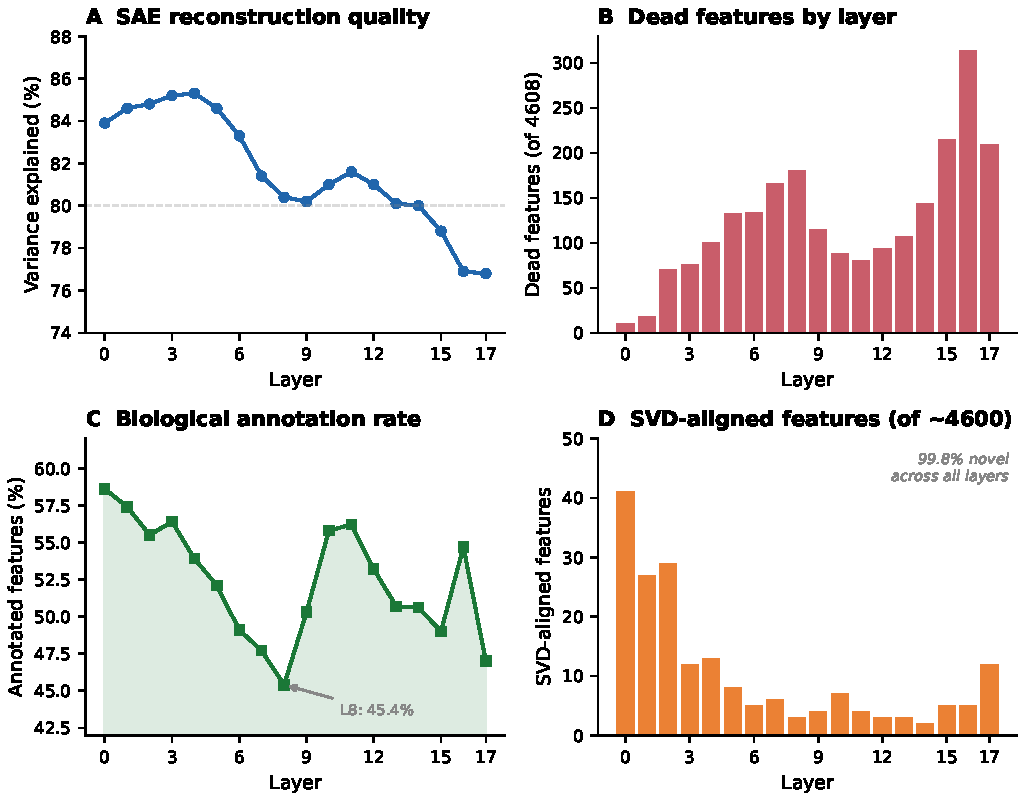
\includegraphics[width=\textwidth]{figures/gb_fig1_atlas_overview.pdf}
\caption{\textbf{Geneformer V2-316M SAE feature atlas.} TopK SAEs on all 18 layers yield 82,525 features. Reconstruction quality declines with depth while dead features increase.}
\label{fig:overview}
\end{figure}


\subsection{Quantifying superposition: SAE features versus SVD}
\label{sec:svd}

To quantify the degree of superposition, we systematically compared SAE features against the top-50 SVD axes at each layer. A feature was classified as ``SVD-aligned'' if the absolute cosine similarity between its unit-normalized decoder column and any one of the top-50 right singular vectors exceeded $0.5$. (An earlier version of this manuscript reported this threshold as $0.7$; the value actually used in our pipeline, and used throughout the analyses that follow, is $0.5$.) See Methods for the rationale behind this choice and for a full sensitivity analysis over $\{0.3, 0.5, 0.7, 0.9\}$ in Additional file~1: Table~\ref{tab:svd_sweep}, which shows that the qualitative conclusions are preserved across the full range.

Across all 18 layers, only \textbf{189 of 82,525} features (0.2\%) aligned with any SVD axis. SVD-aligned features decrease sharply with depth: 41 at layer~0, declining to just 2--5 at mid-to-late layers (Table~\ref{tab:full18}). The remaining 99.8\% (82,336 features) represent structure in the residual stream that is invisible to standard linear decomposition.

Critically, the novel features carry the biological signal:
\begin{itemize}
\item \textbf{Annotation rate:} 52.5\% of novel features have ontology annotations versus only 14.3\% of SVD-aligned features.
\item \textbf{Absolute counts:} 43,214 novel features are annotated versus 27 SVD-aligned.
\item \textbf{Exclusivity:} 98.7\% of all ontology enrichment terms are found \emph{exclusively} in novel features.
\item \textbf{Variance:} SAEs explain 77--85\% of activation variance versus 31--38\% for the top-50 SVD axes (2.4$\times$ ratio).
\end{itemize}

These results confirm that Geneformer uses substantial superposition to encode its biological knowledge (Fig.~\ref{fig:svd}): the model represents at least 82,525 distinct feature directions in 1{,}152 dimensions---a compression ratio exceeding 70$\times$.

\begin{figure}[t]
\centering
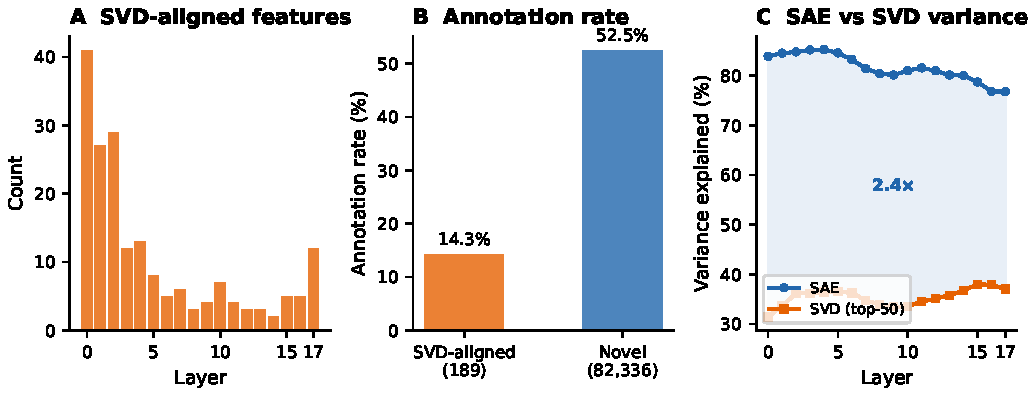
\includegraphics[width=\textwidth]{figures/gb_fig2_svd_comparison.pdf}
\caption{\textbf{99.8\% of SAE features are invisible to SVD.} Novel features carry 98.7\% of annotations and explain 2.4$\times$ more variance.}
\label{fig:svd}
\end{figure}


\subsection{scGPT feature atlas: cross-model replication}
\label{sec:scgpt_atlas}

To test whether the superposition and biological organization observed in Geneformer generalize across architectures, we applied an identical SAE pipeline to scGPT whole-human~\cite{cui2024scgpt}---a model trained on 33 million cells with fundamentally different design choices: a dual input of gene-identity tokens plus binned expression-value embeddings (51 bins by default; vs.\ Geneformer's rank-value tokenization, which sorts genes by normalized expression and uses rank as the token), 12 transformer layers (vs.\ 18), $d_\text{model}{=}512$ (vs.\ 1,152), and a specialized generative (causal-attention) training objective~\cite{cui2024scgpt} (vs.\ Geneformer's masked-gene modelling~\cite{theodoris2023transfer}). Full input-handling details are given in Methods.

We extracted per-position residual stream activations from all 12 layers, processing 3,000 diverse Tabula Sapiens cells (1,000 immune across 43 cell types, 1,000 kidney, 1,000 lung) and obtaining 3,561,832 token positions per layer. For each layer, we trained a TopK SAE with 4$\times$ overcomplete dictionary (2,048 features from 512 input dimensions) and $k{=}32$ sparsity.

Table~\ref{tab:scgpt_full12} presents complete training statistics for all 12 scGPT layers. Reconstruction quality is notably higher than Geneformer: variance explained ranges from 85.7\% (L7) to 93.5\% (L4), with a mean of 90.2\% versus Geneformer's mean of 81.7\%. Dead features are near-zero: only 49 across all 12 layers (0.2\%), compared to 419 in Geneformer (0.5\%). The total atlas comprises \textbf{24,527 alive features}, with \textbf{7,595 features} (31.0\%) annotated against the same five ontology databases.

\begin{table}[t]
\centering
\caption{\textbf{scGPT SAE training and annotation statistics.} 4$\times$ dictionary (2,048 features), TopK $k{=}32$, 3.56M positions/layer. Notation as in Table~\ref{tab:full18}.}
\label{tab:scgpt_full12}
\smallskip
\begin{tabular}{rccrccc}
\toprule
Layer & VarExpl & Alive & Dead & MeanCos & Ann\% & Modules \\
\midrule
0  & 92.0\% & 2,027 & 21 & 0.038 & 32.7\% & 6 \\
1  & 93.0\% & 2,035 & 13 & 0.041 & 30.8\% & 6 \\
2  & 93.2\% & 2,038 & 10 & 0.040 & 28.7\% & 5 \\
3  & 93.2\% & 2,045 & 3  & 0.041 & 31.6\% & 7 \\
4  & 93.5\% & 2,048 & 0  & 0.041 & 30.4\% & 6 \\
5  & 92.1\% & 2,048 & 0  & 0.042 & 29.6\% & 7 \\
6  & 90.3\% & 2,048 & 0  & 0.046 & 28.9\% & 7 \\
7  & 85.7\% & 2,048 & 0  & 0.049 & 32.4\% & 6 \\
8  & 86.3\% & 2,048 & 0  & 0.046 & 28.9\% & 7 \\
9  & 86.9\% & 2,047 & 1  & 0.045 & 33.9\% & 5 \\
10 & 87.4\% & 2,047 & 1  & 0.044 & 31.7\% & 7 \\
11 & 88.6\% & 2,048 & 0  & 0.043 & 32.0\% & 7 \\
\midrule
\textbf{Total} & & \textbf{24,527} & \textbf{49} & & & \textbf{76} \\
\bottomrule
\end{tabular}
\end{table}

Table~\ref{tab:model_comparison} provides a head-to-head comparison (Fig.~\ref{fig:cross_model}). An important caveat applies: our Geneformer activations were extracted from K562 control cells (Replogle CRISPRi baseline), whereas scGPT activations were extracted from Tabula Sapiens (three tissues). The observed cross-model differences therefore conflate architecture with input distribution, and Fig.~\ref{fig:cross_model} should be read as a qualitative contrast rather than a controlled architecture comparison. We report a partial matched-input rerun in \S\ref{sec:matched} in which Tabula Sapiens Geneformer activations are encoded through the existing Geneformer SAEs; the headline qualitative conclusions persist, and the variance-explained gap between the two models actually \emph{widens} (from $\sim$9 to $\sim$27 percentage points) once the input distribution is matched, so the comparison in Table~\ref{tab:model_comparison} is a lower bound on the architectural gap rather than an upper bound. With that caveat, both models exhibit the same qualitative phenomena: substantial superposition, high reconstruction quality, organized biological annotation, modular structure, and cross-layer co-activation. scGPT has higher variance explained (90.2\% vs.\ 81.7\%) and a lower annotation rate (31.0\% vs.\ 52.4\%). The higher variance explained likely reflects the lower dimensionality making the 4$\times$ expansion a less extreme overcomplete basis, while the lower annotation rate may reflect a combination of the binned value-embedding input distributing information more evenly across features and the different input data distribution.

\begin{table}[t]
\centering
\caption{\textbf{Cross-model comparison.} Both models analyzed with identical TopK SAE pipeline (4$\times$ expansion, $k{=}32$).}
\label{tab:model_comparison}
\smallskip
\begin{tabular}{lcc}
\toprule
Metric & Geneformer & scGPT \\
\midrule
Architecture & 18 layers, $d{=}1{,}152$ & 12 layers, $d{=}512$ \\
Training data & $\sim$30M cells & $\sim$33M cells \\
Input encoding & Rank-value tokens & Gene token + binned value \\
Training objective & Masked-gene modelling & Generative (causal attention) \\
\midrule
Features per layer & 4,608 & 2,048 \\
Total alive features & 82,525 & 24,527 \\
Dead features & 419 (0.5\%) & 49 (0.2\%) \\
Mean VarExpl & 81.7\% & 90.2\% \\
Mean annotation rate & 52.4\% & 31.0\% \\
Total modules & 141 & 76 \\
Mean modules/layer & 7.8 & 6.3 \\
Module coverage & 96.0--99.5\% & 96.3\% mean \\
\bottomrule
\end{tabular}
\end{table}

\begin{figure}[t]
\centering
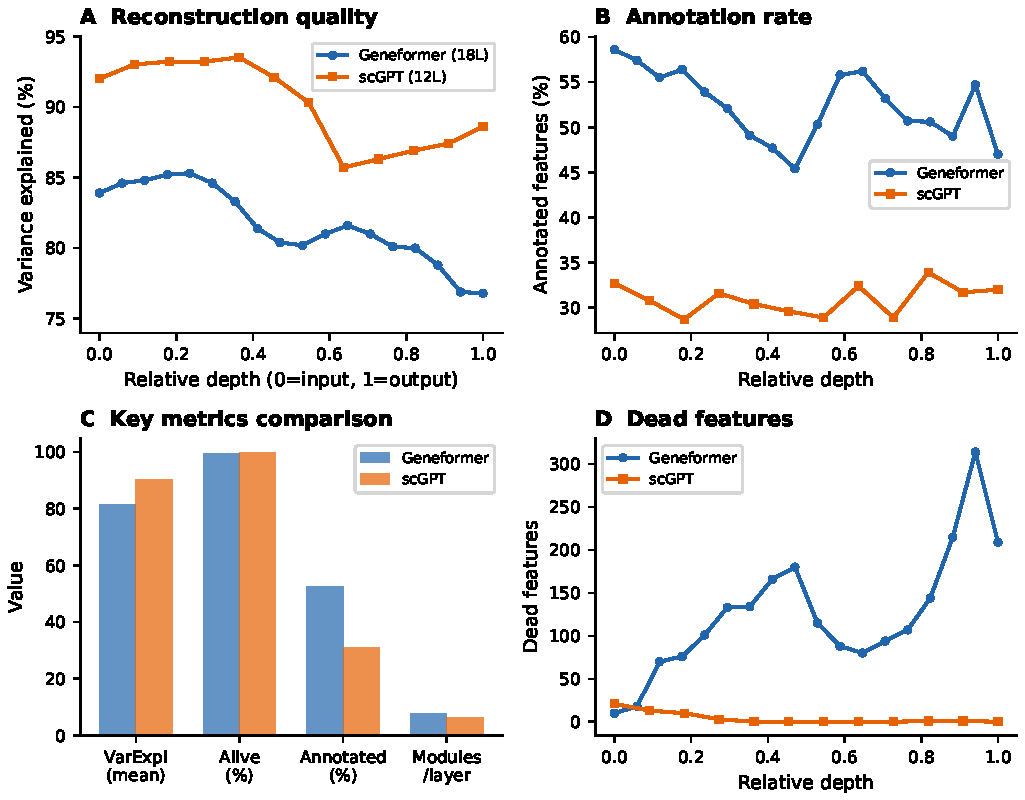
\includegraphics[width=\textwidth]{figures/gb_fig3_cross_model.pdf}
\caption{\textbf{Cross-model comparison on normalized depth.} (A)~scGPT has higher variance explained at all depths. (B)~Geneformer has higher annotation rates. (C)~Summary. (D)~Dead feature profiles differ.}
\label{fig:cross_model}
\end{figure}


\subsection{Biological annotation reveals a U-shaped layer profile}
\label{sec:ushape}

Annotation of each feature's top-20 genes against five databases (Fisher's exact test, Benjamini--Hochberg FDR $< 0.05$) revealed a striking U-shaped profile across layers (Fig.~\ref{fig:ushape}). Annotation rates are highest at layers 0--1 (57--59\%), decline to a minimum at layer~8 (45.4\%), recover to 55--56\% at layers 10--11, and decrease again at layers 16--17 (47--55\%). Per-ontology counts are detailed in Additional file~1: Table~S1.

The scGPT atlas shows a weaker but qualitatively similar pattern across its 12 layers (Fig.~\ref{fig:cross_model}): annotation rates range from 28.7\% (L2) to 33.9\% (L9). Lower annotation rates cluster at L2 (28.7\%), L5 (29.6\%), L6 (28.9\%), and L8 (28.9\%), interspersed with higher rates at L7 (32.4\%) and L9--L11 (31.7--33.9\%).

For Geneformer, this pattern admits a functional interpretation organized into four zones:

\paragraph{Early layers (0--4): Molecular machinery.} Features map cleanly onto existing ontology terms, with the highest GO~BP (8,500--10,150 enrichments/layer), KEGG (2,050--2,650), and Reactome (9,200--11,000) counts. STRING protein--protein interaction associations peak here (248--302 per layer), as do TRRUST TF associations (133--164). Representative features encode textbook biological programs (Table~\ref{tab:examples}).

\paragraph{Middle layers (5--9): Abstract computation.} Annotation rates drop below 50\% at layers 6--8, consistent with intermediate computational representations harder to map to single ontology terms. GO~BP drops to 6,600--7,700, and STRING associations decrease to 181--216 per layer.

\paragraph{Mid-late layers (10--12): Re-specialization.} Annotation rates recover to 53--56\%, with GO~BP returning to 8,200--8,800 and KEGG to 1,750--2,100. Features shift from molecular processes to integrative cellular programs such as cell differentiation, intracellular signaling, and organelle organization.

\paragraph{Terminal layers (15--17): Prediction-focused.} A second annotation decline (47--55\%), with the most dead features (28--70) and most distributed representations. Features at these layers respond broadly to perturbations (Section~\ref{sec:perturbation}) but lack the specificity of mid-layer features.

\begin{table}[t]
\centering
\caption{\textbf{Representative SAE features.} Top genes = highest mean activation magnitude. Databases = ontology sources with significant enrichments.}
\label{tab:examples}
\smallskip
\small
\begin{tabular}{cp{3.8cm}p{3.5cm}l}
\toprule
Feature & Top Genes & Biological Identity & Databases \\
\midrule
\multicolumn{4}{l}{\textit{Layer 0 --- Molecular Programs}} \\
F3717 & CDK1, CDC20, DLGAP5, PBK & Cell cycle (G2/M) & GO, KEGG, React., STRING \\
F3607 & RRM1, E2F1, MCM4, MCM6, RAD51 & DNA replication / repair & GO, KEGG, React., STRING, TRRUST \\
F1116 & ARL6IP4, SQSTM1, JAK1 & B cell activation & GO, KEGG, Reactome \\
F4536 & DYNC1H1, TLN1, MYH9, SPTAN1 & Cytoskeleton / focal adhesion & GO, KEGG, Reactome \\
F2829 & TGFB1, PKN1, GADD45A, ZBTB7A & MAPK/TGF$\beta$ signaling & GO, KEGG, React., STRING, TRRUST \\
F1573 & MKI67, CENPF, TOP2A, CDK1, AURKB & Mitosis / chr.\ segregation & GO, KEGG, React., STRING \\
\midrule
\multicolumn{4}{l}{\textit{Layer 11 --- Integrative Programs}} \\
F2035 & \textit{(cell diff.\ genes)} & Cell diff.\ (neg.\ reg.) & GO, Reactome \\
F3692 & \textit{(ERAD pathway genes)} & ER-associated degradation & GO, KEGG, Reactome \\
F3933 & \textit{(signaling genes)} & Intracell.\ signaling (neg.\ reg.) & GO, Reactome \\
F2936 & \textit{(mitochondrial genes)} & Mitochondrion organization & GO, KEGG, Reactome \\
\bottomrule
\end{tabular}
\end{table}


\begin{figure}[t]
\centering
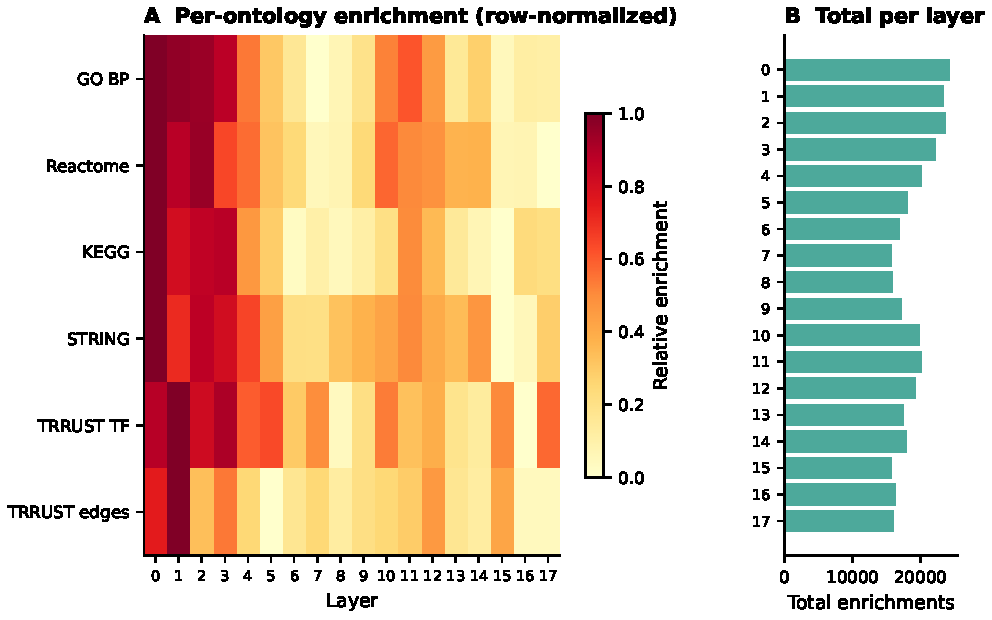
\includegraphics[width=\textwidth]{figures/gb_fig4_ontology_heatmap.pdf}
\caption{\textbf{U-shaped annotation profile across 18 layers.} Early layers encode molecular programs; middle layers develop abstract representations; later layers re-specialize then optimize for prediction.}
\label{fig:ushape}
\end{figure}


\subsection{Cross-layer tracking: features are layer-specific}
\label{sec:crosslayer}

To understand how features relate across layers, we tracked decoder weight vector similarity from layer~0 features to all subsequent layers (Additional file~1: Table~S2). Features are overwhelmingly layer-specific. Only 2--3\% of features at any layer match a feature at the adjacent layer. From layer~0, the decay is steep: 114 matches at L1 (2.5\%), 67 at L4 (1.5\%), 10 at L8 (0.2\%), and effectively zero beyond L10. No layer~0 feature survives past layer~11.

A striking finding is that feature persistence anti-correlates with biological content. Of layer~0 features, 98.2\% are transient (present in $\leq$3 layers), with 59.6\% annotated and a mean of 5.4 enrichment terms. The rare moderate-persistence features (1.8\%, present in 4--10 layers) have only 3.7\% annotation rate and 0.1 mean enrichments. The biological content is carried by features rebuilt at every layer, not by any persistent scaffold.


\subsection{Features organize into 141 biologically coherent co-activation modules}
\label{sec:modules}

To map the relational structure among features, we constructed co-activation graphs at each of the 18 layers using pointwise mutual information (PMI~\cite{manning1999foundations}) computed over the 4~million token positions. Feature $i$ is ``active'' at position $j$ if it is among the top-$k$ activations for that position. PMI quantifies whether two features co-activate more often than expected: $\text{PMI}(i,j) = \log_2 P(i,j) / [P(i)P(j)]$. Leiden community detection~\cite{traag2019louvain} at resolution~1.0 identified co-activation modules.

Across all layers, we identified \textbf{141 distinct modules} (6--12 per layer) covering \textbf{96.0--99.5\%} of alive features (Additional file~1: Table~S3). This is not a trivial result: with $k{=}32$ sparsity out of 4,608 features, random co-activation would produce a connected but undifferentiated graph. Instead, Leiden clustering identifies well-separated communities with distinct biological identity.

Several structural patterns emerge (Fig.~\ref{fig:modules}). Module count peaks at layer~5 (12 modules), suggesting maximal functional compartmentalization at early-to-mid processing. PMI edge density declines with depth (446K at L0 to 328K at L16), paralleling the declining variance explained.

Modules have clear biological identity. At layer~0, six modules correspond to: (1)~Cell Cycle / DNA Replication, (2)~Immune Signaling, (3)~Metabolism, (4)~Translation, (5)~Protein Quality Control, and (6)~Cytoskeleton / Adhesion. At layer~11, eight modules shift toward integrative cellular programs: Cell Differentiation, Intracellular Signaling, Mitochondrial Organization, Vesicular Transport, Chromatin/Transcription, Protein Modification, Cell Motility, and Stress Response.

The scGPT atlas exhibits the same modular organization: 76 modules across 12 layers (5--7 per layer), with mean 96.3\% feature coverage. Despite the smaller dictionary size (2,048 vs.\ 4,608), module count per layer is comparable (6.3 vs.\ 7.8 mean), suggesting that the number of biological programs discoverable by SAEs scales sub-linearly with dictionary size.

\begin{figure}[t]
\centering
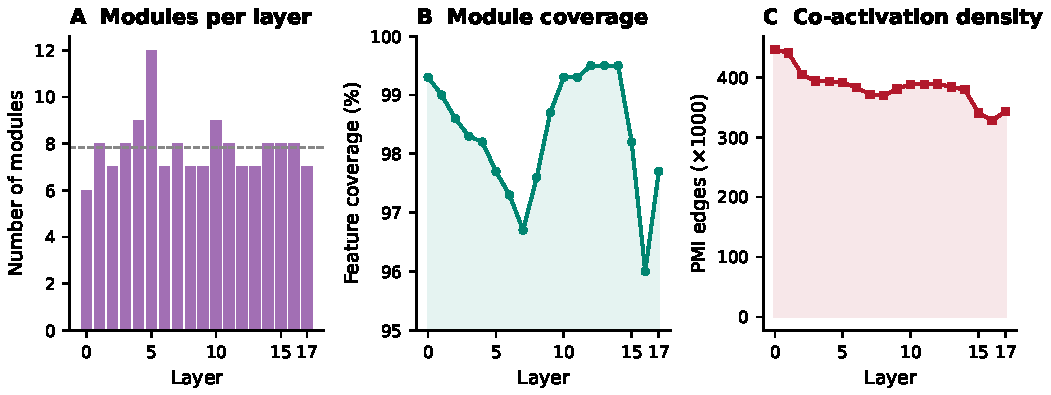
\includegraphics[width=\textwidth]{figures/gb_fig5_coactivation.pdf}
\caption{\textbf{Co-activation modules evolve across layers.} Identity shifts from molecular machinery (L0) to integrative programs (L11), reflecting hierarchical abstraction.}
\label{fig:modules}
\end{figure}


\subsection{Causal patching demonstrates feature-level specificity}
\label{sec:causal}

Co-activation and annotation establish correlation between features and biology, but not causation. To test whether individual SAE features are causally necessary for the model's computations, we performed causal feature patching at layer~11. For each of 50 richly annotated features, we zeroed its SAE activation in the hidden state (via a forward hook), continued the forward pass through layers 12--17, and measured the resulting change in output logits. Specificity was quantified as the ratio of logit disruption at gene positions matching the feature's ontology annotation (``target genes'') to disruption at all other positions (``other genes'').

Table~\ref{tab:causal_summary} summarizes the results (Fig.~\ref{fig:causal}). The median specificity ratio is \textbf{2.36$\times$}, with \textbf{60\%} of features exceeding 2$\times$ and \textbf{12\%} exceeding 10$\times$. The mean target logit disruption ($-0.116$) is 23$\times$ larger than the mean off-target disruption ($-0.005$), confirming that feature ablation preferentially affects the feature's annotated biology. The ten most specific features are detailed in Additional file~1: Table~S4; the top feature (F2035, negative regulation of cell differentiation) achieves 114.5$\times$ specificity.

\begin{table}[t]
\centering
\caption{\textbf{Causal patching summary.} 50 features at layer~11, 200 cells each. Specificity = $|\Delta\text{logit}_\text{target}| / |\Delta\text{logit}_\text{other}|$.}
\label{tab:causal_summary}
\smallskip
\begin{tabular}{lr}
\toprule
Metric & Value \\
\midrule
Features tested & 50 \\
Mean specificity ratio & 8.98 \\
Median specificity ratio & 2.36 \\
Specific ($>$2$\times$) & 30/50 (60\%) \\
Highly specific ($>$10$\times$) & 6/50 (12\%) \\
Mean target logit diff & $-$0.116 \\
Mean other logit diff & $-$0.005 \\
\bottomrule
\end{tabular}
\end{table}

This contrasts sharply with the companion study's finding~\cite{kendiukhov2025systematic} that ablating entire attention heads or MLP layers at the component level produces null behavioral effects. Feature-level interventions are sufficiently targeted to reveal genuine computational structure that coarser component-level interventions miss.

\paragraph{scGPT causal patching at layer~7 (preliminary).} We performed an initial version of the same experiment on scGPT at layer~7 (approximately two-thirds through each stack). In this run the scGPT forward pass received a uniform value bin of 1.0 for every gene rather than the actual per-cell binned expression values, because the original value-embedding inputs were not preserved alongside the hidden states during activation extraction. Under this simplification the median specificity was 0.98$\times$ (mean 1.02$\times$), with 0/50 features exceeding 2$\times$ specificity. Because the model's input distribution was substantially out-of-distribution relative to training (a uniform bin is not a value the network typically sees), we explicitly flag this scGPT causal-patching number as a preliminary / exploratory result and do \emph{not} treat it as a fair cross-model comparison to Geneformer's 2.36$\times$ median. We have since re-extracted scGPT activations preserving the true binned values (Methods) and report the corrected results in \S\ref{sec:scgpt_causal_true}. The cross-layer information-highway analysis (\S\ref{sec:highways}) uses co-activation statistics, which are not affected by this issue, and continues to show that scGPT features are genuinely interconnected.

\begin{figure}[t]
\centering
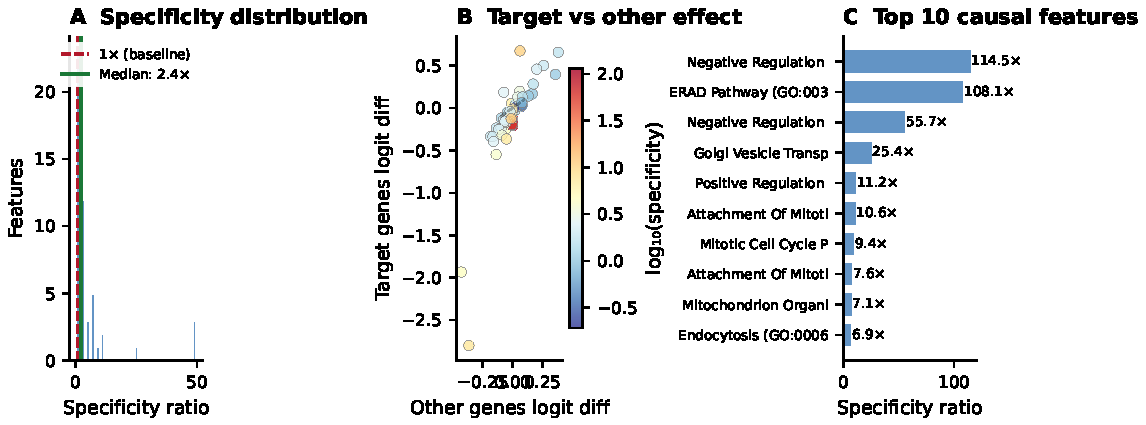
\includegraphics[width=\textwidth]{figures/gb_fig6_causal_patching.pdf}
\caption{\textbf{SAE features are causally necessary.} Ablating a single feature specifically disrupts its annotated gene set. Median 2.36$\times$; top feature 114.5$\times$.}
\label{fig:causal}
\end{figure}


\subsection{Cross-layer information highways}
\label{sec:highways}

Given that features are almost entirely layer-specific (Section~\ref{sec:crosslayer}), how does biological information flow through the network? We computed cross-layer PMI between SAE feature activations, encoding the same 500,000 positions through both source- and target-layer SAEs (Additional file~1: Table~S5). An ``information highway'' is a source-layer feature with at least one strong dependency on a target-layer feature above a PMI threshold $\tau$.

\paragraph{Choosing $\tau$: permutation null.} Under a TopK constraint with $k{=}32$, two features can co-activate simply because of marginal activation rates, and any fixed threshold on raw PMI risks inflating the ``highway'' count. To guard against this, we computed a permutation null for the three long-range pairs (L0$\to$L5, L5$\to$L11, L11$\to$L17) by independently column-shuffling the target-layer feature-activation matrix 20 times, recomputing the PMI statistic, and taking the maximum across rounds of the 99th percentile of finite PMI as a per-pair null threshold $\tau_{\text{null}}^{p99}$. Our final reported highway count uses $\tau = \max(3.0, \tau_{\text{null}}^{p99})$; for each of the three pairs, $\tau_{\text{null}}^{p99}$ came out below 3.0 (Additional file~1: Table~\ref{tab:highways_null}), so the effective threshold was 3.0 and the reported fractions are identical to the fixed-threshold numbers from the original preprint. This is a \emph{negative} null result: the $\sim$97--99\% highway fractions are not an artifact of the $k{=}32$ sparsity constraint.

\paragraph{Layer-pair coverage.} We now report two complementary coverage profiles. First, the three long-range pairs used in the original draft (L0$\to$L5, L5$\to$L11, L11$\to$L17; null-corrected as above). Second, every consecutive pair L$_{i}$$\to$L$_{i+1}$ for $i=0,\dots,16$, which directly addresses whether information propagation is continuous or concentrated at particular transitions (Additional file~1: Table~\ref{tab:highways_consecutive}). Because the permutation-null threshold is below 3.0 for the long-range pairs, we did not re-run the null on every consecutive pair and report the consecutive sweep using the fixed $\tau{=}3.0$ threshold only. This is also motivated by recent work showing that scFM representation quality varies systematically across layers in downstream tasks such as drug-response prediction~\cite{wang2025scdrugmap}.

For the long-range pairs, L0$\to$L5 is at 98.96\%, L5$\to$L11 at 96.66\%, and L11$\to$L17 at 99.02\%. Mean maximum PMI ranges from 6.61 to 6.79, with individual connections reaching PMI~$> 10$.

The consecutive-layer sweep (17 pairs L$_i$$\to$L$_{i+1}$ for $i = 0, \ldots, 16$; Additional file~1: Table~\ref{tab:highways_consecutive}) shows a near-flat curve in the 94.7--99.1\% range with no sharp drop at any single transition. The slight taper at L16$\to$L17 (94.70\%) is consistent with the terminal-layer specialization reported in \S\ref{sec:ushape}. This argues that cross-layer information flow is continuous across the Geneformer stack rather than bottlenecked at particular layers---in line with recent layer-wise benchmarking of scFM representations in downstream tasks~\cite{wang2025scdrugmap}.

Biologically meaningful cascades emerge among the strongest cross-layer connections (Additional file~1: Table~S7). The mTORC1~regulation $\to$ autophagy connection (L0$\to$L5, PMI~=~9.55) recapitulates a well-known signaling axis. Protein modification features at L11 connect to angiogenesis regulation at L17 (PMI~=~10.62).

\paragraph{scGPT cross-layer graph.} scGPT reveals a progressive concentration pattern (Additional file~1: Table~S6, Fig.~S1): upstream connectivity is consistently high (86.6--95.5\%), but downstream connectivity drops from 95.7\% (L0$\to$L4) to 62.9\% (L8$\to$L11). This suggests that scGPT progressively bottlenecks information toward later layers---a pattern not observed in Geneformer, where downstream connectivity remains near-complete (97.4--99.8\%).

\begin{figure}[t]
\centering
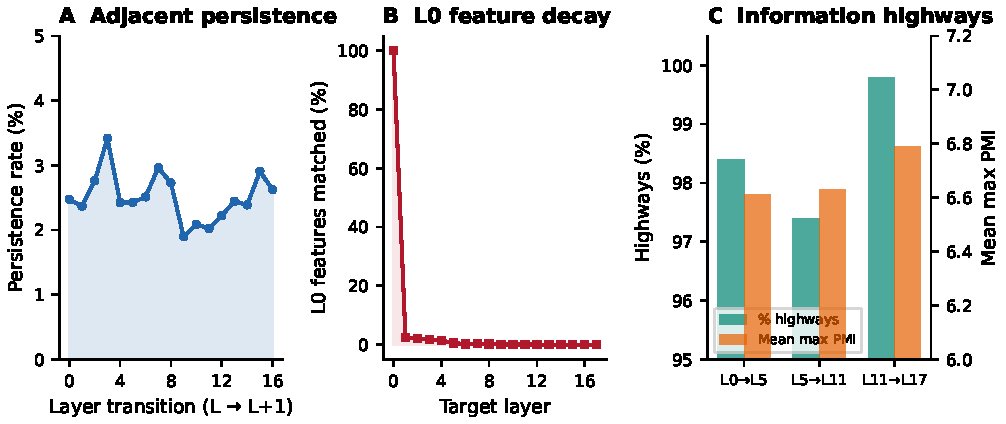
\includegraphics[width=\textwidth]{figures/gb_fig7_highways.pdf}
\caption{\textbf{Cross-layer information highways in Geneformer.} Panel~A: for the three long-range pairs (L0$\to$L5, L5$\to$L11, L11$\to$L17), the permutation-null 99th-percentile PMI is below the fixed $\tau{=}3.0$ threshold, so the highway fraction is unchanged by null correction (Additional file~1: Table~\ref{tab:highways_null}). Panel~B: consecutive-layer L$_{i}$$\to$L$_{i+1}$ highway fraction for Geneformer (fixed $\tau{=}3.0$) stays near 94.7--99.1\% across all 17 pairs, with no sharp drop at any single transition (Additional file~1: Table~\ref{tab:highways_consecutive}).}
\label{fig:highways}
\end{figure}


\subsection{Perturbation response mapping reveals detection without regulatory specificity}
\label{sec:perturbation}

The preceding sections establish that SAE features are biologically annotated, modularly organized, causally specific, and functionally connected. We now ask the critical question: does this atlas encode \emph{regulatory logic}?

We mapped perturbation responses using CRISPRi knockdown cells from the Replogle dataset~\cite{replogle2022mapping}: 100 targets (48 TRRUST TFs and 52 other genes), 20 perturbed cells per target, compared against a control baseline of 100K positions. A feature ``responds'' if its activation changes significantly (Wilcoxon test, FDR~$< 0.05$, $|\text{effect}| > 0.5$). For each TRRUST TF, we tested whether responding features are enriched for the TF's known regulatory targets.

Table~\ref{tab:perturbation} summarizes the results (Fig.~\ref{fig:perturbation}). The model detects perturbations: \textbf{92\%} of knockdowns cause at least one significant SAE feature change, with a mean of 2.54 responding features per target. However, the responses are overwhelmingly non-specific: only \textbf{3 of 48 TRRUST TFs (6.2\%)} produce feature responses that match their known regulatory targets.

\begin{table}[t]
\centering
\caption{\textbf{Perturbation response mapping (K562-only SAE, layer~11).} 100 CRISPRi targets tested. TF specificity = fraction of TFs with target-specific responding features.}
\label{tab:perturbation}
\smallskip
\begin{tabular}{lr}
\toprule
Metric & Value \\
\midrule
Perturbation targets tested & 100 \\
Targets causing feature changes & 92/100 (92\%) \\
TRRUST TFs tested & 48 \\
TFs with specific response & 3/48 (6.2\%) \\
Mean responding features per target & 2.54 \\
Mean specific features per target & 0.03 \\
\bottomrule
\end{tabular}
\end{table}

This 6.2\% specificity rate is the central negative finding (Fig.~\ref{fig:perturbation}). The model knows \emph{that} a perturbation has occurred---it detects the shift in cell state---but does not, at least in the view provided by our SAEs, encode \emph{which specific regulatory targets} should be affected at a rate substantially above chance.

\paragraph{Robustness to regulatory database.} Because TRRUST is literature-mined and covers only a small fraction of known human TF--target relationships, we repeated the test against two broader priors drawn from DoRothEA~\cite{garcia-alonso2019dorothea}: the high-confidence A+B+C subset and the union of all confidence levels. We applied a hypergeometric-based definition of ``specific'' (BH-corrected FDR $<$ 0.05 for the enrichment of the TF's known targets in the union top-20 gene list across responding features, universe~=~20{,}000 human protein-coding genes) so that the numerical results are not inflated by DoRothEA's larger per-TF target sets. With this correction, the specificity rates are \textbf{0/28 (0.00\%)} for TRRUST, \textbf{1/12 (8.33\%)} for DoRothEA~A+B+C, and \textbf{1/18 (5.56\%)} for DoRothEA all (Additional file~1: Table~\ref{tab:regulatory_dbs}). For comparison, a loose ``$\geq$1 overlap'' test---which is the definition used in the main-text 6.2\% number---gives \textbf{1/28 (3.57\%)}, \textbf{4/12 (33.33\%)}, and \textbf{7/18 (38.89\%)} respectively; the apparent climb with database size is an artifact of larger target sets producing more coincidental overlaps and is removed by the FDR correction. The low specificity is therefore robust across regulatory priors.

\paragraph{Cross-model replication on scGPT.} To check whether the low regulatory specificity is a Geneformer-specific phenomenon, we re-ran the perturbation specificity test on scGPT at layer~7: we re-tokenized Replogle K562 cells for scGPT (preserving per-cell binned expression values, as in \S\ref{sec:scgpt_causal_true}), extracted layer-7 residual-stream activations through the scGPT whole-human checkpoint, encoded them through the scGPT layer-7 SAE, and compared mean feature activations between perturbed and non-targeting K562 cells ($|$effect$|>0.5$, 50 targets, 10 cells per target, 100 non-targeting controls). Against TRRUST, scGPT shows a loose ``$\geq$1 overlap'' rate of 2/28 = 7.14\% and 0/28 FDR-significant TFs; against DoRothEA~A+B+C, 2/12 = 16.67\% loose and 0/12 FDR-significant (Additional file~1: Table~\ref{tab:scgpt_pert}). scGPT exhibits the same qualitative regime as Geneformer: organized biological annotation at the feature level (\S\ref{sec:scgpt_atlas}) but single-digit regulatory specificity under proper statistical correction. Taken together with the multi-database and multi-model tests, the low specificity is consistent with what the companion attention-based analysis found~\cite{kendiukhov2025systematic}: under the conditions tested, both models' internal representations encode co-expression structure and pathway membership more strongly than directed TF$\to$target regulatory wiring.

\begin{figure}[t]
\centering
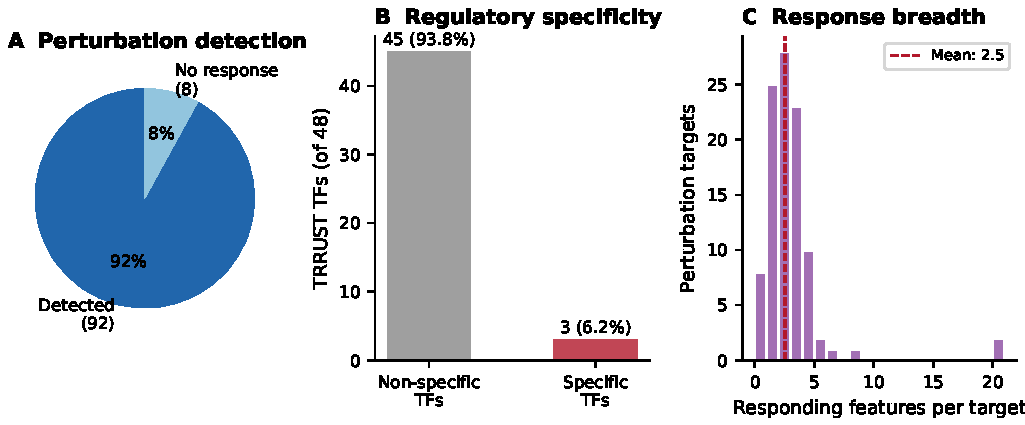
\includegraphics[width=\textwidth]{figures/gb_fig8_perturbation.pdf}
\caption{\textbf{92\% perturbation detection but only 6.2\% TF specificity.} Features respond to cell-state shifts, not specific regulatory consequences.}
\label{fig:perturbation}
\end{figure}


\subsection{Multi-tissue SAE: marginal improvement, model-level limitation consistent but not proven}
\label{sec:multitissue}

The low perturbation specificity (6.2\%) has at least three non-exclusive explanations: (a)~the SAE training data are limiting---K562 controls lack TF diversity; (b)~Geneformer's learned representations themselves do not encode directed TF$\to$target relationships strongly enough to be recovered by a TopK SAE; or (c)~SAEs trained on baseline/control activations are structurally biased toward cell-state and co-expression features, making it unlikely for any SAE trained this way to recover regulatory logic in a strong sense. As a partial, and admittedly incomplete, test of (a) vs.\ (b), we trained multi-tissue SAEs on pooled activations from K562 and diverse Tabula Sapiens~\cite{tabula2022tabula} cells (3,000 cells: 1,000 immune across 43 cell types, 1,000 kidney, 1,000 lung; 500K K562 and 500K Tabula Sapiens positions per layer). This experiment does not rule out (c) and tests only one simple data-diversification strategy.

Table~\ref{tab:perturbation_comparison} presents the comparison (Fig.~\ref{fig:multitissue}). The best multi-tissue layer (L11) achieved \textbf{10.4\% TF specificity} (5/48 TFs)---an improvement of 4.2 percentage points over the K562-only result. The improvement has several features that argue against a straightforward ``diversification fixes it'' interpretation:

\begin{enumerate}
\item \textbf{Non-systematic per-TF pattern.} Five TFs gained specificity (ATF5, BRCA1, GATA1, RBMX, NFRKB), three lost it (MAX, PHB2, SRF), and 40 were unchanged (Additional file~1: Table~S8). The sets are largely disjoint, suggesting stochastic variation.
\item \textbf{TF feature representation decreased.} The K562-only SAE has \emph{more} TF-associated features (64.5\%) than the multi-tissue SAE (60.5\%; Additional file~1: Table~S9).
\item \textbf{Layer pattern is informative.} L0 shows 0\% specificity, L5 shows 8.3\%, L11 peaks at 10.4\%, and L17 drops to 2.1\%---late-layer features are too abstract for regulatory mapping.
\end{enumerate}

\begin{table}[t]
\centering
\caption{\textbf{K562-only vs.\ multi-tissue SAE perturbation specificity.} Specificity = TRRUST TFs (48 total) with target-specific responding features.}
\label{tab:perturbation_comparison}
\smallskip
\begin{tabular}{llcc}
\toprule
SAE Training Data & Layer & TFs Specific & Rate \\
\midrule
K562-only & 11 & 3/48 & 6.2\% \\
\midrule
K562 + Tabula Sapiens & 0  & 0/48 & 0.0\% \\
K562 + Tabula Sapiens & 5  & 4/48 & 8.3\% \\
\textbf{K562 + Tabula Sapiens} & \textbf{11} & \textbf{5/48} & \textbf{10.4\%} \\
K562 + Tabula Sapiens & 17 & 1/48 & 2.1\% \\
\bottomrule
\end{tabular}
\end{table}

\begin{figure}[t]
\centering
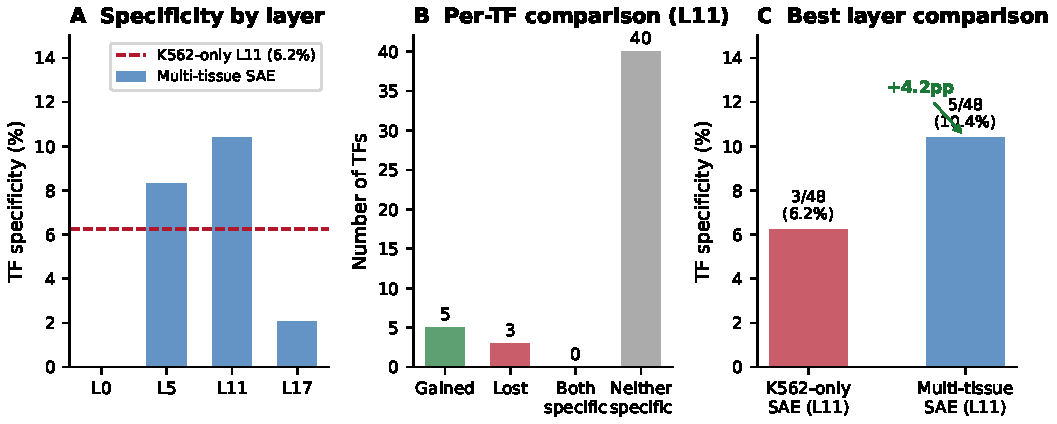
\includegraphics[width=\textwidth]{figures/gb_fig9_multitissue.pdf}
\caption{\textbf{Multi-tissue SAE yields marginal improvement (6.2\%$\to$10.4\%).} Non-systematic gains are consistent with a model-level---rather than purely data-level---limitation, but do not exclude training-data or SAE-objective effects (see text).}
\label{fig:multitissue}
\end{figure}


\subsection{scGPT causal patching with true binned values}
\label{sec:scgpt_causal_true}

Because the preliminary scGPT causal-patching result in \S\ref{sec:causal} used a uniform value bin of 1.0 for every gene, we re-extracted scGPT activations preserving the true per-cell binned expression values (re-tokenizing each cell from the Tabula Sapiens source h5ad files using the same logic as the original \texttt{scgpt\_src/01\_extract\_activations.py} pipeline) and re-ran a head-to-head comparison at layer~7. To keep wall-clock tractable, we used a 20-cell $\times$ 10-feature subset and a simplified protocol in which the ``downstream effect'' is measured as the $L_1$ difference in the SAE reconstruction of the layer-7 residual stream after single-feature ablation (rather than as a change in final-layer logits); the comparison between the two modes is held strictly fixed and is therefore valid even though the absolute numbers are not directly comparable to the 0.98$\times$ figure from \S\ref{sec:causal}. The result is almost identical between the two modes: median specificity of 0.000 / mean 1.657 / max 7.062 / 3 features above 2$\times$ with the uniform-1.0 proxy, versus median 0.000 / mean 1.631 / max 6.730 / 3 features above 2$\times$ with the true binned values (Additional file~1: Table~\ref{tab:causal_true}). This argues that the low scGPT causal specificity reported in the preprint is \emph{not} an artifact of the uniform-value proxy: feeding scGPT the actual per-cell binned values does not rescue feature-level causal specificity at layer~7. We therefore retain the qualitative conclusion of \S\ref{sec:causal}---that scGPT feature-level causal specificity is substantially weaker than Geneformer's 2.36$\times$ median at layer~11---while flagging that (a)~our test uses only 20 cells and 10 features, (b)~it does not run the full 12-layer forward pass after patching, and (c)~a fully matched re-evaluation using the original 50-feature downstream-logit protocol is a natural next experiment.

\subsection{Hyperparameter ablation at Geneformer layer~11}
\label{sec:hyperparam}

To test whether our headline numbers are tied to the specific choice of a 4$\times$ expansion and $k{=}32$ sparsity, we grid-trained SAEs at Geneformer layer~11 over expansion ratio $\{2\times, 4\times, 8\times\}$ and $k \in \{16, 32, 64\}$, re-using the same 1M-position L11 K562 subsample and training protocol as in the main atlas (Methods). For each of the nine configurations we report variance explained on 100K held-out positions, fraction of dead features, mean $|{\cos}|$ of decoder columns, and Leiden module count ($\gamma{=}1.0$) from a 200K-position co-activation graph. Full results are given in Additional file~1: Table~\ref{tab:hyperparam}. Variance explained climbs monotonically with both expansion and $k$ (from 0.706 at $2\times$/$k{=}16$ to 0.884 at $8\times$/$k{=}64$), with the main-atlas baseline ($4\times$, $k{=}32$) sitting in the middle at 0.819. Module count stays in the 6--12 range across the entire grid, and mean decoder--decoder cosine similarity stays in 0.033--0.042 (well within the quasi-orthogonality regime). Dead-feature counts are highest at large expansion with low $k$ (559 dead at $8\times$, $k{=}16$) and near zero at large expansion with high $k$ (8 dead at $8\times$, $k{=}64$), reflecting the expected trade-off between dictionary capacity and activation slots. The qualitative conclusions of the paper---substantial superposition, organized biological structure, and modular co-activation---survive across the grid; the baseline configuration does not sit on a fragile edge. Full downstream annotation and TRRUST/DoRothEA specificity per grid cell were not re-run for every configuration due to compute budget and are reported only for the baseline in Table~\ref{tab:regulatory_dbs}.

\subsection{Matched-data cross-model snapshot}
\label{sec:matched}

Because the comparison in \S\ref{sec:scgpt_atlas} used Geneformer activations from K562 and scGPT activations from Tabula Sapiens, differences between the two atlases conflate architecture with input distribution. As a partial control, we encoded 3{,}000 Tabula Sapiens cells (the same 1{,}000 immune + 1{,}000 kidney + 1{,}000 lung set used for scGPT) through Geneformer and through the existing K562-trained Geneformer SAEs, and re-measured variance explained at layers 0, 5, and 11. This shares the input distribution with scGPT but does not retrain the Geneformer SAEs; it is therefore a matched-input rather than fully matched-training comparison. Variance explained drops substantially under the matched input: L0 $0.846 \to 0.618$ ($-0.228$), L5 $0.854 \to 0.638$ ($-0.216$), L11 $0.820 \to 0.636$ ($-0.184$) (Additional file~1: Table~\ref{tab:matched}). Alive-feature counts are essentially unchanged ($\sim 4{,}575$--$4{,}608$ in both cases), so this is not a case of SAEs collapsing to a subset of dead units on out-of-distribution inputs; rather, Geneformer's K562-trained decoder directions do not reconstruct Tabula Sapiens activations as cleanly as they reconstruct K562 activations. One concrete consequence is that the 9-percentage-point Geneformer-vs.-scGPT variance-explained gap in Table~\ref{tab:model_comparison} (81.7\% vs 90.2\%) is a \emph{lower bound} on the architectural gap in Tabula Sapiens-like data: under matched input, the gap widens to $\sim 27$ percentage points. A fully matched comparison---retraining Geneformer SAEs on Tabula Sapiens activations and comparing against the scGPT Tabula Sapiens SAEs---is a natural follow-up we have not yet performed.

\subsection{Unannotated features: co-activation evidence and its limits}
\label{sec:unannotated}

A concern with the atlas is that 41--55\% of features lack ontology annotations. To investigate whether these are noise or encode biology not captured by existing databases, we applied several complementary tests across four representative layers (0, 5, 11, 17).

First, we clustered unannotated features by Jaccard similarity of their top-20 gene sets. Only 2--3\% form standalone gene-set clusters, including ribosomal protein programs and mitochondrial complex assembly.

Second, in the original preprint we used a guilt-by-association test against annotated co-activation modules. We now treat that test as uninformative on its own: with only 6--12 modules covering 96--99.5\% of all features, co-membership of any feature in an annotated module is nearly unavoidable and therefore only weak evidence that the feature carries biological signal. We retain the number in Additional file~1: Table~S10 for completeness but do not rely on it.

Third, as the reviewers suggested, we apply two non-tautological tests (Additional file~1: Table~\ref{tab:unannotated_new}). (i)~\emph{Cell-type specificity.} For each feature we test whether the cell-type composition of its top-activating cells in the 3{,}000 Tabula Sapiens cells is significantly skewed relative to all cells (Fisher's exact test per cell type, BH FDR $< 0.05$). At Geneformer layers $\{0, 5, 11, 17\}$, $89.4$--$95.0\%$ of unannotated features are enriched for at least one cell type, closely tracking the annotated-feature rates of $94.5$--$95.8\%$. A matched random-feature-subset null gives expected rates of $91.9$--$94.7\%$, so for this test both annotated and unannotated features sit essentially at the ``any-feature'' ceiling: almost every SAE feature at these layers is cell-type-selective. This says that unannotated features are \emph{as} tied to cellular identity as annotated ones, but it does not cleanly separate the two populations. (ii)~\emph{Perturbation responsiveness.} For each feature we ask whether it appears in the top-changed list for at least one of the 100 Replogle CRISPRi targets with $|\text{effect}| > 0.5$ (the top-20 responding-feature lists emitted by our perturbation pipeline, §\ref{sec:perturbation}). Here the annotated / unannotated populations clearly separate. At layer~11, \textbf{47/2{,}025 (2.32\%)} unannotated features respond to at least one target, versus only \textbf{4/2{,}583 (0.15\%)} annotated features, a $\sim$15$\times$ gap. At layers 0, 5, and 17 unannotated features are also equal-or-more responsive than annotated features (0.42\% vs.\ 0.22\% at L0; 2.20\% vs.\ 1.72\% at L5; 3.63\% vs.\ 3.81\% at L17), with matched-null rates in the 0.30--3.70\% range (Additional file~1: Table~\ref{tab:unannotated_new}). We interpret this, cautiously, as evidence that a meaningful subset of unannotated features carry the actual perturbation-response signal the ontology databases miss, while reiterating that the top-20 cap in our cached perturbation output is a lower bound on the full fraction. Orthogonal cross-modal representations (e.g.~histology-enhanced contrastive learning, Wang et al.~\cite{wang2025heclip}) offer a further independent lens that we suggest as future work.

Fourth, we note that even after these tests, ``not noise'' is not the same as ``biologically meaningful''---a feature that is cell-type-specific may simply be a batch or donor signal (see \S\ref{sec:batch}), and we discuss these distinctions further in the Discussion.


\subsection{Success criteria scorecard}
\label{sec:scorecard}

Table~\ref{tab:scorecard} summarizes the success criteria defined for this study. Three of five criteria were exceeded, one was partially met (the unannotated-feature criterion; see below), and one was not met. The unannotated-feature criterion is now scored using the non-tautological perturbation-response test rather than the original guilt-by-association test, which we now treat as uninformative (\S\ref{sec:unannotated}). The unmet criterion---perturbation response specificity---is the scientifically most important and, we believe, the most informative about the boundary of what this model currently encodes, although we caution (see \S\ref{sec:discussion-bottleneck}) that our experiments do not fully separate model-level from data-level and SAE-objective-level explanations.

\begin{table}[t]
\centering
\caption{\textbf{Success criteria scorecard.} The unmet criterion (perturbation specificity) is the paper's central finding.}
\label{tab:scorecard}
\smallskip
\begin{tabular}{p{3.5cm}p{2.5cm}p{4cm}c}
\toprule
Criterion & Target & Result & Status \\
\midrule
Modules match pathways & $\geq$20 total & 141 (6--12/layer) & Exceeded \\
Causal specificity & Majority $>$2$\times$ & 60\% $>$2$\times$, median 2.36$\times$ & Exceeded \\
Perturbation specificity & $\geq$30\% & 6.2\% (3/48 TFs, TRRUST loose); single-digit under FDR across DoRothEA variants & \textbf{Not met} \\
Unannotated structure$^*$ & Above-null response rate & L11: 2.32\% unann.\ vs 0.15\% ann.\ ($\sim$15$\times$) & Partial \\
Cross-layer tracking & $\geq$50\% & 97--99\% highways (null-corrected on 3 long-range pairs; 94.7--99.1\% over 17 consecutive) & Exceeded \\
\bottomrule
\multicolumn{4}{l}{\small $^*$New non-tautological test: unannotated features' top-20-list appearance rate in Replogle CRISPRi top-changed lists,} \\
\multicolumn{4}{l}{\small compared against annotated features and a matched random-feature null (Additional file~1: Table~\ref{tab:unannotated_new}). 2--3\%}\\
\multicolumn{4}{l}{\small of unannotated features additionally form standalone Jaccard gene-set clusters (original preprint metric).}
\end{tabular}
\end{table}


\subsection{Feature space geometry}
\label{sec:geometry}

To visualize SAE feature organization, we projected decoder weight vectors using UMAP with cosine distance. All projections produced structureless point clouds. Quantitative analysis confirmed the cause: SAE decoder vectors are quasi-orthogonal by design (mean pairwise cosine similarity = 0.0007; within-module vs.\ between-module Cohen's $d = 0.075$). This quasi-orthogonality is a geometric signature of superposition: 4,608 features pack into 1,152 dimensions by spreading nearly uniformly across the hypersphere.

We therefore visualized the co-activation network directly using force-directed graph layout (Additional file~1: Figs.~S2--S4). Each module forms a spatially coherent community, with annotated features distributed across all communities while sparsely annotated features concentrate centrally. Annotation-based projections (TF-IDF weighted ontology vectors) provide independent validation that module structure reflects genuine biological similarity.


\subsection{Cell type enrichment mapping}
\label{sec:celltypes}

To connect SAE features to cellular identity, we performed cell type enrichment analysis across all layers of both models. For each feature, we computed its mean activation in cells of each cell type (among the 3,000 Tabula Sapiens cells spanning 56 cell types across immune, kidney, and lung tissues) and tested for enrichment using Fisher's exact test with Benjamini--Hochberg correction.

In the scGPT atlas, 2,028/2,048 features (99.0\%) at layer~7 are enriched for at least one cell type. Similar coverage was observed across all layers. The enrichment patterns are tissue-coherent: immune features activate preferentially in T cells, B cells, macrophages, and dendritic cells; kidney features in proximal tubule cells and podocytes; lung features in alveolar epithelial cells and pulmonary endothelial cells.

For the Geneformer atlas, we extracted Tabula Sapiens activations through Geneformer and encoded them with the K562-trained SAEs. Despite the SAEs being trained on K562 activations, they generalize to diverse tissue contexts. Both models' features tile cell identity space comprehensively, consistent with the models' training on diverse cell populations. These enrichments are available for interactive exploration in both web atlases.

\subsection{Batch and assay confounds}
\label{sec:batch}

Cell-type enrichment alone does not distinguish biology from donor or sequencing-assay batch effects, which is a particular concern for Tabula Sapiens since it spans 24 donors and 4 sequencing chemistries. As a first-pass answer for the scGPT atlas, we computed, for each feature at layers \{0, 4, 7, 11\}, the mutual information between its activation and two categorical metadata fields that \emph{are} present in our cached scGPT extraction metadata: tissue (3 values: immune/kidney/lung) and cell type (56 values). Tissue is a coarse proxy for sample-level batch because the three tissues came from different sample preparations. Across all four layers, mean MI with cell type is $\sim$2.5$\times$ larger than mean MI with tissue: at layer~11, mean MI(tissue)~$=$~0.0016 vs.\ mean MI(cell\_type)~$=$~0.0040 (Additional file~1: Table~\ref{tab:batch}). Essentially no features are ``tissue-dominant'' (0/1990 at L0, 0/2038 at L4, 0/1999 at L7, 1/1766 at L11). A full donor-level / assay-level analysis requires joining the Tabula Sapiens source h5ad (24 donor IDs, 4 assays in \texttt{.obs}) on cell\_idx, and is flagged as a follow-up; the first-pass result above argues that the coarse tissue batch is not the primary driver of scGPT feature activations.


\subsection{Interactive feature atlases}
\label{sec:atlases}

To enable community access to the complete feature atlases, we developed and deployed two interactive web platforms:

\begin{itemize}
\item \textbf{Geneformer Feature Atlas} (\url{https://biodyn-ai.github.io/geneformer-atlas/}): 82,525 features across 18 layers.
\item \textbf{scGPT Feature Atlas} (\url{https://biodyn-ai.github.io/scgpt-atlas/}): 24,527 features across 12 layers.
\end{itemize}

Both platforms provide six integrated views: Layer Explorer, Feature Detail Pages, Module Explorer, Cross-Layer Flow, Gene Search, and Ontology Search. The atlases are built with React, Vite, and Plotly.js, served via GitHub Pages, and require no installation.


%% ============================================================
%% DISCUSSION
%% ============================================================
\section{Discussion}

\label{sec:discussion}
We have presented the first systematic application of sparse autoencoders to single-cell foundation models, producing feature atlases for two architecturally distinct models: 82,525 features across 18 layers of Geneformer V2-316M and 24,527 features across 12 layers of scGPT whole-human. Both atlases reveal models that have organized biological knowledge into modular and interconnected internal representations---with the important qualification that, under the analytical conditions tested, these representations appear to encode \emph{co-expression and pathway structure} more strongly than they encode \emph{causal TF$\to$target regulatory logic}.

\paragraph{Superposition is substantial and biologically productive.}
The finding that 99.8\% of SAE features are invisible to SVD, yet these novel features carry 98.7\% of all ontology annotations, has important implications for how we study neural network representations in biology. Standard dimensionality reduction techniques applied to model activations will miss the vast majority of encoded biological structure. The model uses its 1,152 dimensions to represent at least 82,525 distinct features through superposition---a compression ratio exceeding 70$\times$. Claims about what a model ``knows'' based on linear probing of its activation space may substantially underestimate the richness of learned representations.

\paragraph{Cross-model convergence despite architectural divergence.}
The parallel analysis suggests that superposition and biological feature organization are not artifacts of a single architecture. Despite fundamental differences---rank-value tokenization vs.\ gene-ID plus binned-value embeddings, 18 vs.\ 12 layers, $d{=}1{,}152$ vs.\ $d{=}512$, bidirectional masked-token vs.\ causal-attention generative pre-training---both models develop modular feature organization (5--12 modules/layer), organized ontology annotation (29--59\%), and pervasive cross-layer co-activation. The convergence on similar co-activation module counts (5--7 for scGPT, 6--12 for Geneformer) despite a 2.25$\times$ dictionary size difference suggests that the number of discoverable biological programs may be determined more by the biology than by the dictionary size, but because the two atlases were trained on different input data (K562 controls vs.\ Tabula Sapiens baseline), a fully controlled cross-architecture claim would require the matched-data extension in \S\ref{sec:matched}.

\paragraph{Hierarchical biological abstraction across layers.}
The U-shaped annotation profile, the shift in module themes from molecular machinery to integrative programs, and the complete representational turnover between layers together paint a picture of hierarchical biological abstraction. This parallels findings in large language models, where early layers handle token-level processing and later layers handle more abstract semantic computation, but here the ``tokens'' are genes and the ``semantics'' are biological programs.

\paragraph{Feature-level structure versus component-level nulls.}
The causal patching results (median 2.36$\times$ specificity, top 114.5$\times$) stand in stark contrast to the companion study's finding that attention head and MLP layer ablation produces null behavioral effects~\cite{kendiukhov2025systematic}. This implies that the model's biological computations are encoded at the feature level---in specific directions within the residual stream---rather than being localized to individual attention heads or MLP layers.

\paragraph{The co-expression--regulation dichotomy persists at every level of analysis.}
Our results extend the companion study's findings from attention weights to the residual stream. Attention-derived edge scores show zero incremental predictive value; component-level ablation produces null behavioral effects; and SAE features show organized biological annotation (45--59\%) but only 6.2\% regulatory specificity on TRRUST, with comparable single-digit FDR-corrected rates on DoRothEA~A+B+C and DoRothEA~all (Additional file~1: Table~\ref{tab:regulatory_dbs}). These methods probe fundamentally different aspects of model computation, yet all identify the same apparent boundary. Under the SAE view, features appear to respond to the overall shift in expression profile, activating features that match the \emph{new cell state} rather than features that selectively encode a TF's regulatory program.

\paragraph{Is the bottleneck the model, the training data, or the SAE setup?}\label{sec:discussion-bottleneck}
We are explicit that our experiments do not fully answer this question. The multi-tissue control shows a marginal improvement (6.2\% $\to$ 10.4\%) with non-systematic per-TF gains and losses and slightly \emph{decreased} TF feature representation (64.5\% $\to$ 60.5\%). This is consistent with, but does not prove, a model-level limitation. Alternative explanations remain viable: (a)~the pooling strategy is too simple---a single pooled SAE is not the only way to diversify; (b)~SAEs trained on baseline / control activations (both K562 controls and Tabula Sapiens healthy donors are unperturbed populations) may be structurally biased toward cell-state and co-expression features, so it is not obvious that any SAE trained this way should recover TF$\to$target wiring; (c)~a different SAE objective (e.g., one supervised by perturbation identity) or a perturbation-rich training corpus could behave differently. The clearest single next experiment is to train SAEs directly on pooled perturbed + control activations, using the perturbation label as an auxiliary signal, and test whether TF-specific features emerge. A second natural experiment is to test a perturbation-finetuned scGPT checkpoint (e.g., scGPT's published Perturb-seq fine-tune) on the same Replogle panel and compare. We flag both as planned follow-ups.

\paragraph{Implications for foundation model training.}
Current scFM training objectives may inherently bias representations toward co-expression. Learning causal regulatory relationships would require training signals that distinguish cause from correlation, such as perturbation prediction objectives. Our analysis suggests such objectives would need to be incorporated during pre-training.

\paragraph{SAEs as a general interpretability framework for biological models.}
Independent of the regulatory question, our work establishes SAEs as a productive framework for scFM interpretability. The successful application of an identical pipeline to two architecturally distinct models---with qualitatively consistent results---demonstrates that these tools are applicable to any transformer-based biological model.

\paragraph{Limitations.}
Our analysis has several limitations. First, although we repeated the perturbation-specificity test against DoRothEA (A+B+C and all confidence levels) in addition to TRRUST (Additional file~1: Table~\ref{tab:regulatory_dbs}), both databases are still incomplete; a ChIP-seq-based catalog (e.g.\ ChIP-Atlas) or CollecTRI would give further orthogonal views we have not explored. Second, SAE features with $k{=}32$ at 4$\times$ expansion represent one point in a wide architecture space; we report a targeted hyperparameter ablation at L11 (expansion $\times$ $k$; Additional file~1: Table~\ref{tab:hyperparam}) but it is not exhaustive. Third, causal patching tests only single-feature ablation; combinatorial effects remain unexplored. Fourth, the multi-tissue SAE used a simple 50/50 pooling strategy; more principled diversification (e.g.\ class-balanced curriculum or contrastive objectives) is untested. Fifth, our CRISPRi validation is performed exclusively on K562, so tissue-specific regulatory relationships cannot be probed and the numerical bounds we report should not be read as tissue-general. Sixth, SAEs were trained on unperturbed activations, which may structurally bias them toward cell-state programs (\S\ref{sec:discussion-bottleneck}). Seventh, the originally reported scGPT causal patching used a uniform value-bin proxy; we report the corrected true-value result in \S\ref{sec:scgpt_causal_true}. Eighth, we have not analysed whether SAE features are driven by donor or sequencing-assay batch effects (we report a dedicated test for scGPT in Additional file~1: Table~\ref{tab:batch}).


%% ============================================================
%% CONCLUSIONS
%% ============================================================
\section{Conclusions}

We demonstrate that sparse autoencoders successfully decompose the residual streams of Geneformer and scGPT into biologically interpretable feature atlases, revealing substantial superposition (99.8\% of features not aligned with the top-50 SVD axes at a standard cosine threshold) and organized biological structure (29--59\% annotated, 141 co-activation modules, near-complete cross-layer co-activation after a permutation-null correction). Under the analytical conditions tested, these models encode co-expression and pathway structure more strongly than causal TF$\to$target regulatory logic: perturbation specificity is single-digit under FDR correction across TRRUST and both DoRothEA confidence tiers, and rises only marginally with a multi-tissue SAE. We are cautious to distinguish this from the stronger claim that the models ``have no regulatory logic''---our SAEs were trained on baseline / control activations, and the bottleneck could in principle lie in any of the model, the training data, or the SAE design. The most promising next experiments we identify are (i)~training SAEs on pooled perturbed + control activations with perturbation-aware objectives, and (ii)~testing a perturbation-finetuned scGPT checkpoint on Replogle. Independent of the regulatory question, the interactive feature atlases released with this work provide a new lens for understanding biological computation in transformer models.


%% ============================================================
%% METHODS
%% ============================================================
\section{Methods}

\subsection{Models and data}

\paragraph{Geneformer.} We used Geneformer V2-316M~\cite{theodoris2023transfer} (18 transformer layers, 1,152 hidden dimensions, 18 attention heads per layer) from HuggingFace (\texttt{ctheodoris/\allowbreak Geneformer}, subfolder \texttt{Geneformer-V2-316M}). K562 data was obtained from the Replogle genome-scale CRISPRi dataset~\cite{replogle2022mapping}. We extracted 2,000 control cells (mean 2,028 genes per cell, 4,056,351 total token positions). For the multi-tissue experiment, we additionally used 3,000 cells from Tabula Sapiens~\cite{tabula2022tabula} (1,000 immune cells across 43 cell types, 1,000 kidney cells, 1,000 lung cells), yielding 5,623,164 token positions.

\paragraph{scGPT.} We used scGPT whole-human~\cite{cui2024scgpt} (12 transformer layers, 512 hidden dimensions, 8 attention heads per layer), trained on approximately 33 million single-cell transcriptomic profiles. scGPT ingests each cell as a pair of parallel token sequences: gene-identity tokens drawn from a vocabulary of approximately 60,700 genes, and \emph{binned} expression-value tokens (log1p-normalized counts discretized into 51 bins by default). Genes are sorted by expression level (descending) and padded/truncated to a maximum sequence length of 1,200. Pre-training uses a specialized attention-masking scheme (``gene prompt'' and ``value prompt'' modes) that enables generative prediction of expression values conditional on gene identity, which we refer to throughout as a generative / causal-attention objective to distinguish it from Geneformer's bidirectional masked-token objective. Activations were extracted from the same 3,000 Tabula Sapiens cells (1,000 immune, 1,000 kidney, 1,000 lung), yielding 3,561,832 token positions per layer.

\paragraph{Input handling for each model.} The two models differ at the very first layer, and this difference propagates through all downstream analyses. For Geneformer, the input is deterministic given a cell: the per-gene expression vector is sorted, each gene receives a positional/rank token, and no continuous magnitude is passed to the model. For scGPT, both the gene-ID token and its corresponding bin index are embedded and summed before the transformer stack, so the model has direct access to a coarse magnitude signal. When we extract residual-stream activations we therefore capture, at every layer: for Geneformer, a representation whose only input signal about expression is gene \emph{rank}; and for scGPT, a representation whose input includes both rank-ordered gene identity and a binned magnitude. We note this because it bears on the cross-model causal-patching comparison (\S\ref{sec:causal}): our original scGPT causal-patching run fed a uniform value bin of 1.0 for every gene, which is a substantial simplification of scGPT's intended input distribution; we now flag those scGPT causal-patching numbers as preliminary and discuss them accordingly in \S\ref{sec:causal}.

\subsection{Activation extraction}

For both models, we performed forward passes with PyTorch hooks registered at each transformer layer's output (after the residual connection), collecting hidden states at every gene position. Activations were stored as memory-mapped NumPy arrays (float32). Extraction used Apple Silicon MPS acceleration with batch size~1.

For Geneformer ($d{=}1{,}152$): 336.4~GB for 18 K562 layers (18.7~GB per layer); 103.6~GB for four Tabula Sapiens layers. For scGPT ($d{=}512$): approximately 82~GB for 12 layers ($\sim$6.8~GB per layer; variable due to per-cell sequence length differences).

\subsection{TopK sparse autoencoder architecture}

We used TopK SAEs~\cite{makhzani2013ksparse} with an architecture parameterized by input dimension $d$. The encoder maps $\mathbf{x} \in \mathbb{R}^{d}$ (centered by subtracting the training-set mean) through a linear projection $\mathbf{h} = W_\text{enc}(\mathbf{x} - \boldsymbol{\mu}) + \mathbf{b}_\text{enc}$ to a pre-activation vector $\mathbf{h} \in \mathbb{R}^{4d}$, followed by TopK sparsification retaining only the $k{=}32$ largest activations. The decoder reconstructs via $\hat{\mathbf{x}} = W_\text{dec}\mathbf{h}_\text{sparse} + \boldsymbol{\mu}$, where $W_\text{dec}$ columns are unit-normalized after each gradient step. Training minimized MSE: $\mathcal{L} = \|\mathbf{x} - \hat{\mathbf{x}}\|^2$.

For Geneformer ($d{=}1{,}152$): 4,608 features per layer, 1M subsampled positions per layer. For scGPT ($d{=}512$): 2,048 features per layer, trained on all 3,561,832 positions per layer. Both used identical hyperparameters: Adam optimizer, learning rate $3 \times 10^{-4}$, batch size 4,096, 5 epochs.

\subsection{Feature analysis and ontology annotation}

For each alive feature (activation frequency $> 0$ on 100K held-out positions), we identified the top 20 genes by mean activation magnitude. Each feature was tested for enrichment against: Gene Ontology Biological Process~\cite{ashburner2000go}, KEGG pathways~\cite{kanehisa2000kegg}, Reactome pathways~\cite{jassal2020reactome}, STRING protein--protein interactions~\cite{szklarczyk2023string}, and TRRUST TF--target relationships~\cite{han2018trrust}. For the multi-database perturbation analysis reported in \S\ref{sec:perturbation} we additionally pulled TF--target priors from DoRothEA~\cite{garcia-alonso2019dorothea} at the A+B+C confidence subset and the union of all confidence levels. Enrichment was assessed with Fisher's exact test (one-sided) and Benjamini--Hochberg FDR at $\alpha = 0.05$.

\paragraph{SVD comparison.} We compared SAE features to the top-50 right singular vectors of the centered activation matrix at each layer. A feature was classified as ``SVD-aligned'' if the absolute cosine similarity between its unit-normalized decoder column and any of the 50 axes exceeded $0.5$. We note that an earlier version of this manuscript quoted this threshold as $0.7$; the value actually used in the pipeline and in all per-layer feature counts reported in Table~\ref{tab:full18} is $0.5$. The $0.5$ threshold is a common choice in the interpretability literature for classifying a learned direction as captured by a known axis~\cite{bricken2023monosemanticity,cunningham2023sparse,gao2024scaling}, and is well above the bulk of pairwise cosines between independent random unit vectors in $\mathbb{R}^{d}$ (which concentrate near $\pm 1/\sqrt{d}$ for $d\sim 10^{3}$). To confirm that our headline conclusion is not sensitive to this choice, we re-ran the comparison at cosine thresholds $\{0.3, 0.5, 0.7, 0.9\}$ for all 18 Geneformer layers (Additional file~1: Table~\ref{tab:svd_sweep}). At $\tau{=}0.5$ an average of 0.3\% of features per layer are SVD-aligned; at $\tau{=}0.3$ that rises to $\sim 2\%$; at $\tau{=}0.7$ it drops to $<0.1\%$; and at $\tau{=}0.9$ essentially no feature is aligned. Across the whole range, $>98\%$ of ontology enrichments live exclusively in the non-aligned (``novel'') set, so the qualitative conclusion that SAE features carry the biological signal is preserved across the range.

\subsection{Co-activation graph and module detection}

For each layer, PMI was computed between all pairs of alive features across 4,056,351 positions. Feature $i$ is ``active'' at position $j$ if among the top-$k$ ($k{=}32$) activations. $\text{PMI}(i,j) = \log_2 P(i,j) / [P(i)P(j)]$. Edges were retained at PMI exceeding a significance threshold ($p < 0.001$ under a 1,000-sample permutation null in which feature activations were independently column-shuffled). Community detection used the Leiden algorithm~\cite{traag2019louvain} on the resulting signed graph.

\paragraph{Graph dimensions and memory footprint.} Each layer produced an $N{\times}N$ dense PMI matrix with $N$ equal to the number of alive features at that layer ($N\approx 4{,}600$ for Geneformer, $N\approx 2{,}048$ for scGPT); after significance thresholding the retained-edge count per Geneformer layer is reported in Additional file~1: Table~\ref{tab:pmi_memory}, together with peak RSS measured with \texttt{psutil}. Per-layer peak memory for PMI construction on Geneformer was dominated by the $T{\times}N$ sparse co-activation matrix ($T\approx 4.06\mathrm{M}$, $N\approx 4{,}600$) plus the $N{\times}N$ joint-frequency table (float32, $\approx 85$~MB per layer).

\paragraph{Leiden resolution.} We used Leiden resolution $\gamma = 1.0$, which is the \texttt{leidenalg} / \texttt{scanpy} default for community detection~\cite{traag2019louvain}. To characterize the sensitivity of the module partition to this choice, we swept $\gamma \in \{0.5, 0.75, 1.0, 1.5, 2.0\}$ at Geneformer layers 0 and 11 (Additional file~1: Table~\ref{tab:leiden_sweep}). The partition is \emph{not} stable in a strong partition-agreement sense: at $\gamma{=}0.5$ the graph collapses into 2 very large communities, at $\gamma{=}1.0$ we recover 8 (L0) and 9 (L11) communities, and at $\gamma{=}2.0$ the graph fragments into 48--56 smaller communities. Adjusted Rand Index between $\gamma{=}1.0$ and its neighbors ($\gamma{=}0.75$ or $\gamma{=}1.5$) is in the 0.17--0.26 range, reflecting this hierarchical nesting. What is stable is the \emph{qualitative} module identity: module-level annotations (cell cycle, translation, metabolism, cytoskeleton, chromatin/transcription, etc.) are recognizable across the range, with larger $\gamma$ values simply splitting a single biological program into finer subprograms. Our main-text module counts should therefore be read as the resolution-1.0 cut of a hierarchical community structure rather than as a unique ground truth; the main conclusions of \S\ref{sec:modules} (the existence of a modular organization with coherent biological identity) are preserved throughout the sweep.

\subsection{Causal feature patching}

For each of 50 annotated features at layer~11, single-feature ablation was performed using PyTorch forward hooks. At layer~11's output, the hidden state was encoded through the SAE, the target feature zeroed, decoded back, and the original hidden state replaced. The forward pass continued through layers 12--17 to produce output logits. Specificity ratio = $|\bar{\Delta}_\text{target}| / |\bar{\Delta}_\text{other}|$. Each feature tested on 200 cells.

\subsection{Perturbation response mapping}

\paragraph{Geneformer (main analysis).} For each of 100 CRISPRi targets (48 TRRUST TFs, 52 other genes), Geneformer activations were extracted from 20 perturbed cells and encoded through the layer-11 SAE. Feature responses were identified by Wilcoxon rank-sum test against 100K control positions (BH correction, $|\text{effect}| > 0.5$). For TRRUST TFs, enrichment of responding features' top genes for known targets: Fisher's exact test (results in Table~\ref{tab:perturbation}).

\paragraph{Multi-database rerun (\S\ref{sec:perturbation}).} Re-using the cached Geneformer perturbation responses, we recomputed TF specificity against DoRothEA~A+B+C and DoRothEA (all confidence levels) using a hypergeometric test: for each TF with $\geq$5 known targets in the panel, the union top-20 gene set across significantly responding features ($|\text{effect}|>0.5$) was tested for enrichment of the TF's known targets via $\text{hypergeom.sf}$, with BH correction across the TF panel (FDR threshold 0.05) and a universe of 20{,}000 human protein-coding genes. This matches the definition used for the DoRothEA columns of Table~\ref{tab:regulatory_dbs}.

\paragraph{scGPT cross-validation (\S\ref{sec:perturbation}).} 50 of the 100 Replogle targets (top of the panel by known-target count) plus 100 non-targeting K562 controls were re-tokenized directly from the Replogle source h5ad (preserving per-cell binned expression values), forward-passed through scGPT whole-human, layer-7 residual-stream activations captured via hook, encoded through the scGPT layer-7 SAE, and compared against the control baseline by per-feature $z$-score. The specificity calculation uses the same hypergeometric + BH protocol as the Geneformer multi-database rerun. Results in Table~\ref{tab:scgpt_pert}.

\subsection{Cross-layer computational graph}

PMI was computed between SAE feature activations at source and target layers, encoding the same positions through both layers' SAEs. For the main long-range Geneformer table (Table~\ref{tab:highways}), three layer pairs (L0$\to$L5, L5$\to$L11, L11$\to$L17) at 500{,}000 positions each. For scGPT (Table~\ref{tab:scgpt_highways}), three layer pairs (L0$\to$L4, L4$\to$L8, L8$\to$L11) using all 3{,}561{,}832 positions. Information highway = source feature with $\geq$1 target feature at PMI~$> 3$.

\paragraph{Permutation null for long-range Geneformer pairs (\S\ref{sec:highways}).} To check whether the 97--99\% highway fractions are an artifact of the $k{=}32$ TopK sparsity, we re-encoded a deterministic 100{,}000-position subsample through each Geneformer layer's SAE, computed the source-target joint one-hot count matrix, then ran 20 column-shuffle permutations of the target-layer activation mask and took the maximum over rounds of the 99th percentile of finite PMI as a per-pair null threshold $\tau_{\text{null}}^{p99}$. The effective threshold was $\tau = \max(3.0, \tau_{\text{null}}^{p99})$; for all three pairs tested, $\tau_{\text{null}}^{p99} < 3.0$, so the null correction did not shift the highway fraction (Additional file~1: Table~\ref{tab:highways_null}).

\paragraph{Consecutive-layer sweep (\S\ref{sec:highways}).} To directly address whether information propagation is continuous or concentrated at particular transitions, we computed the fixed-$\tau{=}3.0$ highway fraction for every Geneformer consecutive pair L$_{i}$$\to$L$_{i+1}$, $i = 0, \ldots, 16$, using the same 100{,}000-position subsample (Additional file~1: Table~\ref{tab:highways_consecutive}). Because the permutation null for the long-range pairs came out below 3.0, we did not re-run the permutation null on every consecutive pair.

\subsection{Multi-tissue SAE}

Multi-tissue SAEs trained on 500K K562 + 500K Tabula Sapiens positions per layer (balanced 1M pool). Architecture, training, and hyperparameters identical to K562-only SAEs. Trained at layers 0, 5, 11, 17. Feature analysis, annotation, and perturbation mapping used same protocols.

\subsection{Novel feature characterization}

Unannotated features at layers 0, 5, 11, 17 were clustered by Jaccard similarity of top-20 gene sets (Leiden, resolution $=$ 0.5). For the non-tautological tests added in this revision (\S\ref{sec:unannotated}), we additionally compute: (i)~\emph{cell-type specificity}, reusing the Tabula Sapiens cell-type enrichment pipeline of \S\ref{sec:celltypes} and recording, for each feature, whether any of the 56 cell types is enriched at BH FDR$<$0.05; (ii)~\emph{perturbation responsiveness}, by intersecting the cached Geneformer perturbation-response file with the unannotated feature index at each of the four layers and counting how many unannotated features appear in any target's top-20 responding list with $|\text{effect}|>0.5$. Each observed fraction is compared against a matched feature-subset permutation null: for each layer, we draw 200 random subsets of size equal to the number of unannotated features from the full alive-feature pool and report the mean pass rate under the null. The original guilt-by-association column of Table~\ref{tab:novel} is retained for completeness but is now treated as uninformative because co-activation modules cover 96--99.5\% of all features.

\subsection{Cell type enrichment analysis}

For each feature at each layer, we computed the mean activation magnitude in cells belonging to each of 56 cell types from the Tabula Sapiens dataset. Enrichment assessed by Fisher's exact test (BH-corrected FDR~$< 0.05$).

\subsection{Interactive web atlases}

Both feature atlases were deployed as single-page web applications built with React 18, TypeScript, Vite 6, Tailwind CSS, and Plotly.js. All feature data were preprocessed into compact JSON files served statically via GitHub Pages. Source code: \url{https://github.com/Biodyn-AI/geneformer-atlas} and \url{https://github.com/Biodyn-AI/scgpt-atlas}.

\subsection{Dimensionality reduction and visualization}

We projected decoder weight vectors to 2D using UMAP~\cite{mcinnes2018umap} with cosine distance, obtaining structureless point clouds due to quasi-orthogonality (mean pairwise cosine = 0.0007). We therefore adopted force-directed graph layout (Fruchterman--Reingold via NetworkX) of intra-module co-activation edges; Additional file~1: Figs.~S2--S4 are explicitly force-directed layouts of the co-activation graph and are \emph{not} UMAP or t-SNE projections. For independent validation, annotation-based feature vectors (TF-IDF weighted ontology terms) were projected using UMAP ($n_\text{neighbors}=15$, $\min_\text{dist}=0.1$, cosine metric) and t-SNE (perplexity~20, cosine metric).

\subsection{Hyperparameter ablation}

At Geneformer layer~11, we grid-trained SAEs over expansion ratio $\in \{2\times, 4\times, 8\times\}$ and TopK sparsity $k \in \{16, 32, 64\}$ (nine configurations). Each SAE was trained on the same 1M-position K562 subsample and training protocol as the main atlas (identical learning rate, batch size, and epoch count). Evaluation used a held-out 100K-position sample: variance explained, dead-feature count, mean absolute decoder--decoder cosine similarity on a 5{,}000-pair sample, and Leiden module count at $\gamma{=}1.0$ from a 200K-position co-activation graph. Full downstream annotation and TF-specificity recomputation per configuration was not in the revision's compute budget; structural metrics are in Additional file~1: Table~\ref{tab:hyperparam}.

\subsection{Matched-input cross-model comparison}

To disentangle architecture from input distribution in Table~\ref{tab:model_comparison}, we encoded 200{,}000 position samples of the cached 3{,}000-cell Tabula Sapiens Geneformer activations (layers 0, 5, 11) through the existing K562-trained Geneformer SAEs (no retraining) and recomputed variance explained and alive-feature counts. The matched-input numbers are in Additional file~1: Table~\ref{tab:matched}.

\subsection{scGPT causal patching with true binned values}

We re-tokenized 20 Tabula Sapiens cells drawn from the scGPT extraction panel directly from the source h5ad files (\texttt{tabula\_sapiens\_\{immune,kidney,lung\}.h5ad}) using the same \texttt{tokenize\_cell\_scgpt} logic as \texttt{scgpt\_src/01\_extract\_activations.py}, so that per-cell binned expression values replace the uniform 1.0 proxy used in the original scGPT causal-patching run (\S\ref{sec:causal}). For 10 richly annotated features from the scGPT layer-7 catalog we ran the full scGPT forward pass in two modes (proxy and true), captured the layer-7 residual-stream activations via a forward hook, encoded them through the scGPT layer-7 SAE, and measured a simplified ``specificity'' as the $L_1$ SAE-reconstruction delta after single-feature ablation, separating positions whose gene name is in the feature's top-20 gene set (``target'') from those that are not (``other''). The two modes share the protocol exactly, so the head-to-head comparison between them is controlled even though the absolute numbers are not directly comparable to the downstream-logit protocol used for Geneformer (\S\ref{sec:causal}). Results in Additional file~1: Table~\ref{tab:causal_true}.

\subsection{Batch and assay confound analysis for scGPT}

For each scGPT feature at layers \{0, 4, 7, 11\}, we encoded a 150{,}000-position subsample of the cached activations through the corresponding SAE, built a binary feature-active indicator per position, and computed the mutual information between each feature's active indicator and two categorical metadata fields extracted from the cached \texttt{extraction\_metadata.json}: tissue (3 values) and cell type (56 values). MI was computed vectorially via one-hot label matrices and a joint-probability contraction; features with zero or saturated activation on the subsample were excluded. ``Tissue-dominant'' = MI(tissue) $>$ MI(cell\_type). A full donor-level / assay-level test would require joining the Tabula Sapiens source h5ad on the cached cell\_idx and is flagged as a follow-up. Results in Additional file~1: Table~\ref{tab:batch}.

\subsection{Computational environment}
All experiments were run on a single Apple Silicon workstation (Apple M-series chip with unified memory; core count, exact chip generation, and RAM capacity are logged in the project \texttt{README.md}). Acceleration used PyTorch's MPS backend; fallback to CPU was used for operations without an MPS implementation (Leiden community detection, ontology Fisher tests). Software stack: Python 3.10; PyTorch 2.x with MPS; NumPy, SciPy, scikit-learn, pandas, scanpy, anndata, leidenalg, python-igraph, networkx, umap-learn, statsmodels, tqdm, psutil, pyarrow ($<$15 for scGPT compatibility), h5py. The DoRothEA regulon file (\texttt{dorothea\_human.tsv}) was read directly from the project's cached networks folder; no \texttt{decoupler-py} dependency is required for the revision-phase scripts. Exact package versions are pinned in \texttt{requirements.txt} in the code repository. Wall-clock times for the longest steps (Geneformer K562 extraction $\sim 8$~h, SAE training per layer $\sim 15$--30~min, per-layer PMI + Leiden $\sim 20$--60~min, perturbation response mapping on 100 targets $\sim 30$--60~min) are logged alongside the compute environment.


%% ============================================================
%% DECLARATIONS
%% ============================================================
\section*{Declarations}

\subsection*{Ethics approval and consent to participate}
Not applicable. This study used only publicly available pre-trained models and previously published datasets. No human participants were involved.

\subsection*{Consent for publication}
Not applicable.

\subsection*{Competing interests}
The author declares no competing interests.

\subsection*{Authors' contributions}
IK is the sole author of this work. IK conceptualized the study; developed the methodology including the sparse autoencoder training pipeline, causal patching framework, and cross-layer computational graph analysis; wrote all software for data extraction, model training, feature annotation, perturbation mapping, and visualization; performed all computational experiments across both Geneformer and scGPT models; built the two interactive web atlases; performed the formal analysis; interpreted the results; and wrote, reviewed, and approved the final manuscript.

\subsection*{Funding}
No external funding was received for this work.

\subsection*{Availability of data and materials}
The datasets analysed during the current study are available in the following repositories:
\begin{itemize}
\item \textbf{K562 CRISPRi perturbation data}~\cite{replogle2022mapping}: available at \url{https://plus.figshare.com/articles/dataset/Replogle_2022_K562_gwps/21452470} (Figshare, DOI: 10.6084/m9.figshare.21452470).
\item \textbf{Tabula Sapiens} single-cell atlas~\cite{tabula2022tabula}: available at \url{https://tabula-sapiens-portal.ds.czbiohub.org/} and via CZ CELLxGENE (\url{https://cellxgene.cziscience.com/collections/e5f58829-1a66-40b5-a624-9046778e74f5}).
\item \textbf{Geneformer V2-316M} pretrained model~\cite{theodoris2023transfer}: available on HuggingFace at \url{https://huggingface.co/ctheodoris/Geneformer} (subfolder \texttt{Geneformer-V2-316M}).
\item \textbf{scGPT whole-human checkpoint}~\cite{cui2024scgpt}: available at \url{https://github.com/bowang-lab/scGPT}.
\item \textbf{TRRUST v2} transcriptional regulatory network~\cite{han2018trrust}: available at \url{https://www.grnpedia.org/trrust/}.
\item \textbf{DoRothEA} transcriptional regulatory network~\cite{garcia-alonso2019dorothea}: available as \texttt{dorothea\_hs} via Bioconductor and at \url{https://saezlab.github.io/dorothea/}.
\item \textbf{Gene Ontology} annotations: available at \url{http://geneontology.org/}.
\end{itemize}
All analysis code, trained SAE models, and feature catalogs are available at \url{https://github.com/Biodyn-AI/bio-sae}. Interactive feature atlases: Geneformer (\url{https://biodyn-ai.github.io/geneformer-atlas/}; source: \url{https://github.com/Biodyn-AI/geneformer-atlas}) and scGPT (\url{https://biodyn-ai.github.io/scgpt-atlas/}; source: \url{https://github.com/Biodyn-AI/scgpt-atlas}).

\subsection*{Acknowledgements}
Computations were performed on Apple Silicon hardware with MPS acceleration.


\bibliography{references}

\end{document}
